%--------------------------------------------------------------------------- 

%                           der Universität Münster
%                         http://cvpr.uni-muenster.de
%
%---------------------------------------------------------------------------
% Geeignet für:
%  - Seminararbeiten
%  - Bachelorarbeiten
%  - Masterarbeiten
%---------------------------------------------------------------------------
% Autoren:
%  - Daniel Tenbrinck
%  - Fabian Gigengack
%  - Michael Schmeing
%  - Lucas Franek
%  - Andreas Nienkötter
%---------------------------------------------------------------------------
% Version:
%  - 1.0.3 (05.10.2016)
%	 - Ersetzung von veralteten Befehlen durch Aktuelle
%	 - Einige ausführlichere Beispiele
%    - Einführung von listings
%    - Aktuelle Version der Eidesstattlichen Erklärung
%  - 1.0.2 (09.09.2011)
%    - Titelblatt um Matrikelnummer und Studiengang ergänzt
%  - 1.0.1 (05.07.2011)
%---------------------------------------------------------------------------
% 
% "THE BEER-WARE LICENSE" (Revision 42):
% The above mentioned authors wrote this file. As long as you retain this
% notice you can do whatever you want with this stuff. If we meet some day,
% and you think this stuff is worth it, you can buy us a beer in return.
%  --------------------------------------------------------------------------

\documentclass[a4paper, twoside, 12pt, ngerman]{scrbook} % Layout-Einstellungen für das Dokument

\usepackage[utf8]{inputenc} % UTF-8 Codierung
\usepackage[ngerman]{babel} % Deutsche Beschriftung

\usepackage{graphicx} % Um Bilder einzufügen
\usepackage{wrapfig} % Wrapping figures
% \usepackage{subfigure} % Um mehrere Bilder in eine figure einzufügen
\usepackage{subcaption}
\usepackage{amssymb, amsmath} % Für Mengensymbole und über Gleichheitszeichen schreiben
\usepackage{verbatim} % Um Quellcode in das Dokument einzufügen.
\usepackage{xcolor} % Für Farben
\usepackage[linkbordercolor=blue]{hyperref} % Für Links im Dokument
\usepackage{cleveref} % Einfachere Referenzen auf andere Sektionen des Dokuments
\usepackage{algorithmic} % Für Pseudo-Code
\usepackage{algorithm} % Wrapper für Pseudo-Code
\usepackage{enumitem}% http://ctan.org/pkg/enumitem
\usepackage[font={small}, labelfont=bf]{caption} % kleine Bildunterschriften
\usepackage{geometry} % Für Feinanpassungen des Layouts
\usepackage[autostyle=true,german=quotes]{csquotes}
\usepackage{listings} % Für Code-Listings
\renewcommand{\lstlistingname}{Quelltext} %Ändert die Überschrift von Listing nach Quelltext
\newcommand{\reg}[1]{\[\text{#1}\]}
\newcommand{\el}[1]{\enquote{\textit{#1}}} % Kommando für Spezielle Namen aus LimeSurvey oder ODM
\newcommand{\jv}[1]{\textit{#1}} % Kommando für Spezielle Namen aus LimeSurvey oder ODM
% Einstellungen für Abstand an den Rändern
\geometry{a4paper,left=35mm,right=35mm,top=20mm,bottom=20mm, includeheadfoot}

\setitemize{font=\bfseries, leftmargin=2cm}
\usepackage[sorting=none]{biblatex}
\addbibresource{Quellen.bib}

\begin{document}
\pagenumbering{roman}

% Titelblatt
\begin{titlepage}
\begin{centering}
\vspace*{\fill}

\includegraphics[width=12cm]{./img/wwu-logo-neu.pdf}

\vspace{2cm} 

{\Large
	\textbf{Design eines Mappings und Implementierung eines Converters von LimeSurvey Umfragen und Antworten in CDISC ODM}\\[1.2cm]
}

{\large
	Bachelorarbeit\\[2cm]
}

{\large
	vorgelegt von:
}

{ \Large
	\textbf{Antonius Johannes Mende}\\[1cm]
}

{\large
	Matrikelnummer: 461 328\\[2mm]
}

{\large
	Studiengang: Informatik 1.FB\\[1cm]
}
    
{\large
	Thema gestellt von:
}

{\Large
	\textbf{Dr. Ludger Becker}\\[1cm]
}
                               
{\large
	Arbeit betreut durch:
}

{\Large
	\textbf{Dr. Ludger Becker und Dr. Tobias Brix}\\[1cm]
}

{\large
Münster, \today
}
\vfill
\end{centering}

\end{titlepage}

% Inhaltsverzeichnis
\tableofcontents

\cleardoublepage
\pagenumbering{arabic}

% Die Hauptkapitel der Arbeit
\chapter{Einleitung}
\label{ch:einleitung}

Das Thema dieser Arbeit ist die Konvertierung von LimeSurvey Archiven in das Operational Data Model.
LimeSurvey ist ein Werkzeug, mit dem man einfach Umfragen erstellen kann, welche dann wiederum von beliebig vielen Teilnehmern beantwortet werden können.
Umfragewerkzeuge lassen sich sehr vielseitig einsetzen, um die Meinungen von Kunden, Patienten oder jedem anderen Menschen einzuholen.
Gerade in den heutigen Zeiten, wo immer mehr Daten gesammelt und verarbeitet werden können, ist es wichtig, Kompatibilität zwischen verschiedenen Werkzeugen und Formaten herstellen zu können.
Das Institut für Medizinische Informatik an der WWU ist eine der vielen Institutionen, welche LimeSurvey nutzt, um die Meinungen und Erfahrungen von Patienten einzuholen.

\section{Problem}
Der XML-Standard lässt dem Programmierer sehr viel Freiheit, was das Design eines XML-Formates angeht. Dadurch sind verschiedene XML-Formate im Regelfall nicht kompatibel beziehungsweise untereinander austauschbar.
Das macht es notwendig, XML-Dokumente zu konvertieren, um ein Dokument in einem Format mit einem Werkzeug nutzen zu können, welches nur ein anderes XML-Format unterstützt.
Als Zielformat wird ODM-XML von CDISC verwendet.
ODM wurde mit dem Ziel entwickelt, den Austausch und die Archivierung von Forschungsdaten und anderen damit verbundenen Daten zu ermöglichen.
Durch die Unabhängigkeit des Formates von spezifischen Plattformen oder Firmen wird es durch weit mehr Werkzeuge unterstützt als ein Format wie LSA, welches von LimeSurvey selbst und zu deren eigenen Zwecken entwickelt wurde.
Dies sieht man auch an dem Institut für Medizinische Informatik, welche dieses Projekt betreuen.
Dort wird ODM täglich zur Verwaltung klinischer Daten genutzt, gleichzeitig ist aber auch LimeSurvey das Umfragewerkzeug der Wahl, um Daten von Patienten zu sammeln.
Diese gesammelten Daten müssen dann exportiert und konvertiert werden, um sie in bestehenden Systemen einpflegen zu können.

\section{Ziel}
Ziel der Arbeit ist es, genau darzustellen, wie man aus einem LimeSurvey Archiv in ein ODM Dokument umwandeln kann und einen Konverter zu implementieren, welcher das bewerkstelligt.
Es sollen so viele der Forschungsdaten wie möglich übertragen werden, zusätzliche Daten, welche z.B. die Darstellung der Daten betreffen, sollen nicht mit übertragen werden.

% Im Einleitungskapitel werden dem Leser das Thema, die Grundlagen und vergleichbare Arbeiten präsentiert.

% Im Folgenden werden ein paar wichtige Tipps zum Erstellen der wissenschaftlichen Arbeit festgehalten. Die vorliegende inhaltliche Strukturierung dient nur zur Orientierung und ist nicht verbindlich. Insbesondere bei Seminararbeiten kann die Struktur abweichen. Beispielsweise ist dort nicht generell eine Implementierung gefordert (und folglich müssen auch keine Ergebnisse beschrieben werden). Auch Zusammenfassung, Danksagung, eidesstattliche Erklärung, Abbildungs- und Tabellenverzeichnis können bei Seminararbeiten weggelassen werden.


% \section{Referenzierung von Unterkapiteln}
% \label{s:ref} 
% Man sollte direkt jedes Kapitel, Unterkapitel und jede Formel mit einem Label versehen \verb+\label{}+ um eine konsistente Referenzierung im gesamten Dokument zu ermöglichen. Eine Referenzierung im Fließtext lässt sich mittels \verb+\ref{}+ umsetzen.


% \section{Zeilenumbrüche und Absätze}
% \label{s:zeilenumbruch} 
% Zeilenumbrüche sollten im Quelltext immer mittels einer Leerzeile umgesetzt werden, um eine automatische Texteinrückung in der darauffolgenden Zeile zu ermöglichen. Dies macht das Lesen der Arbeit einfacher. Auf die Verwendung des LaTeX-Kommandos \verb+\\+ sollte verzichtet werden.


% \section{Einfügen von Grafiken}
% \label{s:grafik} 
% Grafiken sollten mittels der \verb+\figure+-Umgebung eingebettet werden. Um die Druckqualität und Wiederverwendbarkeit der Grafiken für Vorträge, Poster, etc.\ zu erhöhen sind Vektorgrafiken (z.B.\ .eps oder .pdf) zu bevorzugen. Zur Erzeugung und Konvertierung von Vektorgrafiken ist die OpenSource Software \emph{Inkscape} zu empfehlen.

% Um mehrere Bilder horizontal anzuordnen, sollte die \verb+\subfigure+-Umgebung verwendet werden. Diese Bilder können dann mit \verb+\subref+ oder \verb+\ref+ referenziert werden und erscheinen im Text als \subref{fig:subfig1} oder \ref{fig:subfig1}.

% \begin{figure}
% \begin{center}
% 	\subfigure[Das Logo]{
		% 
\includegraphics[width=0.45\columnwidth]{./img/wwu-logo-neu.pdf}
		% \label{fig:subfig1}
	% }
	% \subfigure[Noch einmal das Logo]{
		% 
\includegraphics[width=0.45\columnwidth]{./img/wwu-logo-neu.pdf}
		% \label{fig:subfig2}
	% }
% \end{center}
% \caption{Das Logo der WWU}
% \label{fig:histogram}
% \end{figure}


% \section{Wissenschaftliches Zitieren}
% \label{s:zitat}
% Für das Referenzieren von wissenschaftlicher Literatur wie Fachbüchern, Konferenzpapern und Veröffentlichungen in Wissenschaftsmagazinen gibt es unterschiedliche Konventionen. Je nach Fachrichtung weichen Layout und Zitationsstil sehr stark voneinander ab \cite{jele2010}. Wir empfehlen aus Gründen der Einheitlichkeit die Verwendung der \emph{Bibtex}-Umgebung. Die zitierte Literatur kann ausgelagert in einer Datei (z.B.: Quellen.bib) gepflegt werden und mittels des \verb+\cite+-Kommandos referenziert werden.


% \section{Zusammenfassung}
% \label{s:zusammenfassung}
% Zum Ende eines längeren Kapitels bietet es sich häufig an eine Zusammenfassung der wichtigsten Punkte zu liefern. Dies erleichtert das Lesen und den Übergang zum nächsten Kapitel.


\chapter{Methodik}
\label{ch:methodik}

\section{Akronyme}

\begin{description}[font=\sffamily\bfseries, leftmargin=0cm, itemsep=-0.15cm, style=nextline]
	\item \textbf{EDC} \el{Electronic Data Capture} Das Sammeln und Verarbeiten von Daten
	\item \textbf{RegEx} \el{Regular Expression} Ein Ausdruck, der genutzt werden kann, um Zeichenketten auf eine bestimmte Struktur zu überprüfen
	\item \textbf{XML} \el{Extensible Markup Language}
	\item \textbf{XSD} \el{XML Schema Definition} Eine Datei, welche beschreibt, wie ein XML-Dokument aufgebaut sein sollte, um einer bestimmten Definition zu entsprechen.
	\item \textbf{SAX} \el{Simple API for XML} Ein Standard, welcher beschreibt, wie man ein XML-Dokument parsen kann. Dieses wird sequentiell eingelesen und für definierte Ereignisse wird eine vorgegebene Rückruf-Funktion aufgerufen. Ein Programm kann eigene Funktionen registrieren und so das Dokument verarbeiten.
	\item \textbf{DOM} \el{Document Object Model} Bietet die Möglichkeit, die Hierarchie der XML-Knoten in Baumform darzustellen und so zu navigieren/ den Baum zu bearbeiten
	\item \textbf{CDISC} \el{Clinical Data Interchange Standards Consortium}
	\item \textbf{CDISC ODM} \el{Operational Data Model} von CDISC entwickeltes XML-Format (siehe \cref{m:odm})
	\item \textbf{lsa} Dateiendung des LimeSurvey Archives (siehe \cref{m:lsa})
	\item \textbf{lsr} Dateiendung der LimeSurvey Response Datei (siehe \cref{m:lsa})
	\item \textbf{lss} Dateiendung der LimeSurvey Struktur Datei (siehe \cref{m:lsa})
\end{description}

\section{LimeSurvey}
% - Umfragewerkzeug, sammeln von Meinungen/Interessen/Entscheidungsgrundlagen
% - Firma gleichen Namens aus D
% - Wird von den Entwicklern in der Cloud-Edition angeboten
% - 4 Pläne
% 	- Free
% 	- Basic (34 Euro/Monat)
% 	- Expert (29Euro/Monat)
% 	- Enterprise (74 Euro/Monat)
% - Code auch Open-Source

LimeSurvey ist ein von der gleichnamigen deutschen Firma entwickeltes Werkzeug für Umfragen.
Laut ihrer Website ist LimeSurvey ein für Einsteiger und Profis sowie für Privatpersonen als auch Institutionen gut geeignetes Werkzeug, um die Meinungen, Interessen und Entscheidungsgrundlagen einer Zielgruppe herauszufinden.
Es wird seit 2006 an der Software entwickelt und sie ist sowohl als Cloud-Edition über die Firma erhältlich, sowie auch als OpenSource-Projekt.\\

Falls man die Cloud-Edition nutzen will, hat man fünf Optionen: \textit{Free}, \textit{Basic}, \textit{Expert}, \textit{Enterprise} und \textit{Corporate}.
Diese unterscheiden sich vor allem durch die Zahl an Antworten pro Monat, die Menge an Upload-Speicher, E-Mail-Support, White-Label-Umfragen, Alias-Domains und die Entfernung des LimeSurvey-Brandings.
Innerhalb der \textit{Corporate}-Lösung kann man noch dedizierte Server und die Nutzung von SAML beantragen.
Preislich bewegt man sich in einem Rahmen von 0€-74€ für die normalen Lösungen und einem individuell absprechbaren Preis für die \textit{Corporate}-Lösung.

\subsection{Features}
\subsubsection{ExpressionScript}
\label{m:expr_script}
Mit Expression Script lässt sich komplexe Logik in die Umfrage einbringen.
Die LimeSurvey-interne Skriptsprache lässt Bedingungen zu, unter denen bestimmte Fragen oder Antworten angezeigt werden sollen.
Man kann hier sowohl Antworten auf vorherige Fragen einbinden, als auch Informationen über den Teilnehmer, welche er vorher angegeben hat beziehungsweise welche über ihn gespeichert wurden.
Man kann mehrere Szenarios designen und es sind Vergleiche mit den Standard-Operatoren sowie RegEx möglich.

\subsubsection{Timings}

Es ist möglich genau festzulegen, wie viel Zeit ein Nutzer zum Beantworten einer Frage hat.
Es können Warnmeldungen zu bestimmten Abschnitten innerhalb der Zeitperiode angezeigt werden, die CSS-Klasse kann angepasst werden und das Beantworten anderer Fragen kann unterbunden werden.

\subsection{Fragegruppen}

% - Name/Beschreibung/Randomisierungsgruppe/Relevanz
% - Kann beliebig viele Fragen enthalten

Fragen in LimeSurvey sind in Fragegruppen unterteilt. Jede Frage ist genau einer Gruppe zugeordnet.
Eine Gruppe kann beliebig viele Fragen enthalten, weiterhin hat sie einen Titel, eine Beschreibung, eine Randomisierungsgruppe und eine Relevanz-Gleichung, wo mittels ExpressionScript (siehe \cref{m:expr_script}) angegeben werden kann, wann die Fragen dieser Gruppe angezeigt werden sollen.
Es darf beliebig viele Fragegruppen geben.

\subsection{Fragetypen}

% - 36 Fragetypen (manche sind keine "Fragen" per se, davon gibt es 28), 5 Gruppen
% - Bedingungen

Es gibt 36 Fragetypen in LimeSurvey, welche in fünf Kategorien unterteilt sind.
Davon sind allerdings nicht alle tatsächlich Fragen, auf die der Teilnehmer antworten kann, insgesamt gibt es vier Fragetypen, welche nicht explizit Fragen sind.
Die möglichen Antworten auf Freitext- und Zahlenfragen lassen sich mittels RegEx limitieren.
Es gibt pro Frage einen optionalen Hilfstext.
Fragen mit vordefinierten Antworten erhalten eine \enquote{Keine Antwort}-Option, wenn sie nicht verpflichtend sind.
Im folgenden sollen alle Typen einmal aufgelistet und kurz beschrieben werden.


\subsubsection{Einfachauswahl}

Auf folgende Fragen kann man maximal eine Antwort geben.
\begin{itemize}
	\item[5 Punkte Wahl] Hier kann auf einer Skala von 1 bis 5 ein Wert ausgewählt werden
	\item[Liste] Hier kann aus einer vordefinierten Liste eine Antwort gewählt werden. Es gibt drei unterschiedliche Darstellungsmöglichkeiten für diese Liste, entweder als Dropdown-Menü, als Bootstrap-Buttons oder mit Radio-Buttons neben den Antworten
	\item[Liste mit Kommentar] Dies ist eine Listen-Frage wie oben, allerdings kann für die Frage auch noch ein Kommentar im Freitext geschrieben werden
	\item[Image-Select-List] Hier wird zu der Liste an Antworten noch ein Bild angezeigt. Die Antworten werden mit Radio-Buttons daneben angezeigt
\end{itemize}

\subsubsection{Matrix}

% - Man kann aus einer Festen Liste an Möglichkeiten eine pro Subfrage Auswählen

Pro Frage gibt es beliebig viele Subfragen, für jede Subfrage kann eine der vordefinierten Antworten ausgewählt werden.
Subfragen werden typischerweise als Zeilen dargestellt, die Antworten als Spalten

\begin{itemize}
	\item[5 Punkte] Hier kann auf einer Skala von 1 bis 5 ein Wert ausgewählt werden
	\item[10 Punkte] Hier kann auf einer Skala vom 1 bis 10 ein Wert ausgewählt werden
	\item[Z/G/A] Hier kann aus den drei Möglichkeiten \enquote{Zunahme/Gleich/Abnahme} eine gewählt werden
	\item[J/N/U] Hier kann aus den drei Möglichkeiten \enquote{Ja/Nein/Unsicher} eine gewählt werden
	\item[Matrix (Custom)] Hier kann eine eigene Liste an Antwortmöglichkeiten definiert werden
	\item[Matrix nach Spalte] Identisch zu Matrix (Custom), allerdings werden Zeilen und Spalten getauscht
	\item[Dual Matrix] Es gibt zwei selbst erstellbare Listen an Antwortmöglichkeiten, man kann aus beiden eine Antwort pro Subfrage wählen
	\item[Matrix (Freitext)] Hier kann man zwei Listen an Subfragen angeben. Daraus wird dann eine Matrix erstellt, wo in jeder Zelle Freitext als Antwort geschrieben werden kann
	\item[Matrix (Zahlen)] Identisch zu Matrix (Freitext), aber es können nur Zahlen als Antwort angegeben werden
\end{itemize}

\subsubsection{Multiple Choice}

Hier können mehrere Antworten aus einer vordefinierten Liste ausgewählt werden.
Optional kann ein \enquote{Anderes}-Feld zugänglich gemacht werden, wo Teilnehmer eine eigene Antwort schreiben können

\begin{itemize}
	\item[Multiple Choice] Darstellung als Bootstrap-Buttons oder Radio-List ist möglich
	\item[Image Select] Hier wird ein Bild mit angezeigt
	\item[Kommentar] hier kann ein Kommentar pro Antwortfeld geschrieben werden
\end{itemize}

\subsubsection{Textfragen}

\begin{itemize}
	\item[Browser Detect] Erkennt den Webbrowser des Teilnehmers. Dies ist keine Frage, welche der Teilnehmer beantworten kann
	\item[Freitext] Hier kann der Teilnehmer einen Text eintippen. Es gibt kurze/lange und riesige Freitexte
	\item[Mehrere Texte] Es gibt mehrere Subfragen. Für jede kann ein kurzer Freitext angegeben werden
	\item[Input on Demand] %TODO
\end{itemize}

\subsubsection{Maskenfragen}

\begin{itemize}
	\item[Datum/Zeit] Hier kann ein Datum und eine Uhrzeit angegeben werden. Das Format ist einstellbar, es kann auch ein minimales Datum angegeben werden
	\item[Ja/Nein] Hier kann mit Ja oder Nein geantwortet werden
	\item[Gleichung] Hier kann ein Text angegeben werden, wo der Nutzer Variablen einträgt, diese können in einer Rechnung verwendet werden, dessen Ergebnis dann angezeigt wird
	\item[Dateiupload] Hier kann eine Datei als Antwort hochgeladen werden
	\item[Geschlecht] Hier kann zwischen \enquote{Männlich}, \enquote{Weiblich} und \enquote{Keine Antwort} ausgewählt werden
	\item[Sprachumschaltung] Hier kann der Teilnehmer die Sprache ändern. Auch das ist keine richtige Antwort
	\item[Zahleneingabe] Hier kann nach einer Zahl als Antwort gefragt werden.
	\item[Mehrfache Zahlen] Hier gibt es mehrere Subfragen, auf die jeweils mit einer Zahl geantwortet werden muss. Die Maximal/Minimal-Werte sind limitierbar, genau so wie auch die Maximal- und Minimal-Summe. Es können genaue Gesamtergebnisse verlangt werden und nur Ganzzahlen als Antwort verlangt werden
	\item[Ranking (Advanced)] Hier kann der Teilnehmer Elemente aus einer vordifinierten Liste sortieren. Es müssen nicht alle Elemente einsortiert werden
	\item[Textanzeige] Hier wird ein Text angezeigt. Auch hier kann nicht geantwortet werden
\end{itemize}

\subsection{Export}
\subsubsection{LimeSurvey Archiv}
\label{m:lsa}
Das LimeSurvey Archiv ist eine von sieben Möglichkeiten, Daten von einer LimeSurvey Umfrage zu exportieren.
Ein solches Archiv ist eine komprimierte Datei im .lsa-Format, welche mehrere extrahierbare Dateien enthält.
Die Zahl und Art der Dateien ist dabei abhängig von den Einstellungen. Zwei Dateien sind immer enthalten:\\
Die erste Datei enthält die Umfrage-Struktur sowie Informationen über die Art und Weise, wie die Fragen darstellt werden sollen (die .lss-Datei), die zweite Datei enthält die Antworten der Teilnehmer (.lsr-Datei).
Ausdrücklich erwähnt wird dabei, dass Dateien, die als Antwort auf eine Frage hochgeladen wurden, nicht Teil des Archivs sind.
Weitere optionale Dateien sind eine Token-Datei, welche Daten über die % TODO

\subsubsection{Weitere Exportmöglichkeiten}
\begin{itemize}
	\item[LSS] Es ist möglich, nur die im LSA enthaltene LSS-Datei zu exportieren, das wird mittels dieser Option gemacht.
	\item[Excel/.csv] Hier sind weitere Einstellungen möglich, wie das Exportieren eines Teils der Antworten oder die Wahl eines bestimmten Formates (Word, Excel, CSV, HTML, PDF).
	\item[SPSS] SPSS ist ein Software-Paket, welches zur statistischen Analyse von Daten genutzt wird. Auch hier kann ausgewählt werden, welche Antworten exportiert werden sollen. Die Nutzung der Open-Source Version PSPP ist auch möglich
	\item[R] R ist eine Alternative zu SPSS, hier werden allerdings alle Daten exportiert
	\item[STATA-xml] Auch STATA ist eine komerzielle Lösung für Datenanalyse wie SPSS. Hierfür werden die Daten von LimeSurvey direkt in das proprietäre STATA-Format umgewandelt.
	\item[VV] Durch \enquote{vertical verfication} ist es möglich, die Antworten zu modifizieren und die modifizierte Datei dann wieder zu importieren
\end{itemize}

\section{ODM}
\label{m:odm}

% - Ein Datenstandard im XML-Format
% - entwickelt von der CDISC
% - Ziel: Ein klares, einheitliches Format für Klinische Daten
% - Zusätzliche Daten wie Metadaten oder admin. Daten werden auch gespeichert
% - Plattform-unabhängig
% - Unabhängig von spezifischen Firmen
% - Mittlerweile viel genutzt in EDC Tools

ODM ist einer der Standards, welcher von CDISC entwickelt wurde, um den gesamten Zyklus einer Studie in ihren verschiedensten Formen zu standardisieren.
Es dient dazu, sowohl Metadaten als auch klinische Daten einer Studie zu erfassen. Auch administrative Daten sind im Standard enthalten.
ODM ist unabhängig von spezifischen Firmen und Plattformen und daher gut zum Austausch zwischen verschiedensten Werkzeugen und Gruppierungen geeignet.
Bereits 2006 hat ODM im internationalen Raum Anklang gefunden, in Deutschland allerdings noch nicht.
Das ändert sich mittlerweile, das IMI der WWU zum Beispiel nutzt das Format bereits in mehreren Werkzeugen.

\subsection{Aufbau}

Zuerst sollte angemerkt werden, dass hier bei weitem nicht alle Elemente, die im ODM-Standard definiert sind, vorgestellt werden. Das hat sowohl Zeit- als auch Platzgründe, weiterhin werden viele Elemente für die Abbildung von LimeSurvey nicht gebraucht.
Für diese Arbeit sind besonders zwei Teile des ODM Standards relevant: Die \el{Study} und die \el{ClinicalData}.
Weiterhin gibt es noch \el{AdminData}, \el{ReferenceData} und \el{Association}.
Grundlegend werden andere Elemente mittels einer OID referenziert, ein Attribut, welches jedes Element besitzt, das man referenzieren kann.

\subsubsection{Study}

Eine Studie hat globale Variablen und grundlegende Definitionen.
Weiterhin gibt es die \el{MetaDataVersion}, wo die Struktur der Umfrage festgelegt wird.
In der einer Version der Metadaten sind alle Elemente in Referenzen und Definitionen aufgeteilt, wobei die Referenzen immer zuerst im nächst \enquote{höhergelegenen} Element vorkommen.\\

Das Basiselement einer Studie ist das \el{Protocol}.
Dies enthält Elemente des Typs \el{StudyEventRef}.
Dann folgen Elemente des Typs \el{StudyEventDef}, welche wiederum Referenzen auf Elemente des Typs \el{FormDef} beinhalten.
Dieses Schema setzt sich noch mit den Elementen \el{ItemGroupDef} und \el{ItemDef} fort.\\

Als weitere Elemente gibt es noch die \el{CodeList} und die \el{Condition}.
In einer \el{CodeList} werden Antwortmöglichkeiten festgehalten, welche auf eine Frage (Element des Typs \el{ItemDef}) gegeben werden können.
Entsprechend enthält \el{ItemDef} ein Element \el{Question}, in welchem eine Frage festgehalten wird.
Mit \el{ConditionDef} kann eine Bedingung festgelegt werden.
Referenziert eine Frage ein Element dieses Typs und evaluiert der Ausdruck zu \enquote{true}, wird die Frage nicht angezeigt.

\subsubsection{ClinicalData}

In der \el{ClinicalData} gibt es für jeden Teilnehmer der Studie ein Element des Typs \el{SubjectData}.
Ab hier ist dann die Stuktur der Studie abgebildet, wobei die \el{ItemData} das unterste Element ist und die Antwort auf eine Frage beinhaltet.

\section{dom4j}

% - API für den Zugriff und die Verarbeitung von XML-Dokumenten
% - Bietet simple Wege, um existierende Funktionen wie XPath oder Parsing mittels DOM/SAX zu nutzen
% - Auch Dokumente erstellen möglich

Dom4j ist eine API, welche die bestehenden Funktionen der \jv{javax}-Bibliothek abstrahiert und so wesentlich simplere Wege bietet, diese zu nutzen.
Unter anderem ist es möglich, Elemente in einem XML-Dokument mittels XPath-Ausdrücken zu finden und DOM/SAX-Parser zu nutzen, um ein Dokument zu verarbeiten.
Auch ein \jv{XMLWriter} existiert, welcher unter anderem Standardelemente von XML automatisch an ein Dokument anhängt und das Format des Dokuments mittels eines einzeiligen Befehls so anpassen kann, dass es leicht für einen Menschen lesbar ist.

%%
%\section{Mathematische Notation}
%\label{s:notation}

%Mathematische Formeln können mittels der \verb+\begin{align}...\end{align}+ Umgebung gesetzt werden:

%\begin{align}
%f(n) & =
%	\begin{cases}
%		n/2, & \text{wenn }n\text{ gerade,}\\
%		3n+1, & \text{wenn }n\text{ ungerade.}
%	\end{cases}
%\label{eq:f} \\
%%
%g(n) & = \frac{n}{2} \label{eq:g}
%\end{align}
%
%\section{Algorithmus}
%\label{s:algorithmus}
%
%Eigene Algorithmen beschreibt man am Besten mit Hilfe von Pseudo-Code und dem Paket \verb+algorithm+.
%
%\begin{algorithm}
%\caption{Algorithmus}
%\label{alg:alg}
%\begin{algorithmic}
%\algsetup{indent=2em}
%
%\REQUIRE Argument $n\in\mathbb{N}$
%\STATE $a = 0$
%\FOR{ $i=0,\dots,n$}
%	\STATE $a = a + 1$
%\ENDFOR
%\RETURN $a$
%\end{algorithmic}
%\end{algorithm}


\chapter{Ergebnisse}
\label{ch:ergebnisse}

\section{Mapping}

\subsection{Dummy Elemente in ODM}

- ODM kann mehr Beziehungen in Studien darstellen
- Es müssen Dummy-Elemente angelegt werden, weil LimeSurvey diese Elemente nicht hat, sie aber in ODM vorkommen müssen
- Betroffen: GlobalVariables, StudyEvent

\subsection{Umfrage-Eigenschaften}

- Eine Umfrage wird als ein \el{Form} dargestellt
- Titel, Beschreibung und ID der Umfrage werden zu Titel, Beschreibung und ID des \el{Forms}

\subsection{Fragegruppen}

- Aus jeder LS Gruppe wird eine ItemGroup in ODM
- Eigenschaften werden 1:1 abgebildet

\subsection{Fragen}

- Aus einer Frage in LS werden pot. mehrere ItemDef's in ODM (fragetypabhängig)
- Elemente aus \el{Questions} und \el{Subquestions} und \el{Question\_l10ns} werden genutzt

\section{Implementierung}

% Dieses Kapitel sollte die Ergebnisse beinhalten, die mit den Methoden aus \autoref{ch:methodik} erstellt wurden.

% \begin{table}[h]
% \caption{Beispieltabelle}
% \begin{center}
% 	\begin{tabular}{|c||c|c|}
% 		\hline
% 		Spalte1 & Spalte2 & Spalte3 \\ 
% 		\hline\hline
% 		   1    &    2    &    3    \\ 
% 		\hline
% 	\end{tabular}
% \end{center}
% \label{tbl:table}
% \end{table}


\chapter{Diskussion}
\label{ch:diskussion}

% In diesem Kapitel werden die zuvor vorgestellten Ergebnisse der Arbeit diskutiert. Häufig wird es mit dem Fazit zusammengelegt.

% Verwandte Arbeiten hier

\section{Auslassen von Fragetypen}
\label{d:leave}

Auch wenn mit diesem Konverter eine vollständige Umsetzung der LimeSurvey Archiv-Daten angestrebt wird, so werden doch einige Fragetypen bewusst nicht umgesetzt.
Im Folgenden soll erläutert werden, welche Fragetypen nicht konvertiert werden, wie diese Fragetypen hätten umgesetzt werden können und warum die Entscheidung getroffen wurde, dies nicht zu tun.

\subsection{Datei-Upload}

Der Fragetyp \el{Datei-Upload} kann genutzt werden, um den Nutzer auf eine Frage mit einer Datei antworten zu lassen.
In ODM hätte man diese Datei einbinden können, indem man sie in \el{hexBinary} umwandelt, ein Datentyp in ODM, welcher Stream-Daten in einem hexacodierten Binärformat sammelt.
Trotzdem wurde dieser Fragentyp im Konverter nicht umgesetzt.
Das liegt zum einen daran, dass die hochgeladenen Dateien nicht Teil des Archives sind (siehe \cref{m:lsa}) und andererseits daran, dass die Praktikabilität dieses Vorgehens eher fragwürdig ist.
Unter anderem wird eine Rekonstruktion zur Originaldatei schwer, da es zum Beispiel keine Informationen über den ursprünglichen Dateityp gibt, auch wird die XML-Datei nur noch sehr unangenehm durch einen Menschen lesbar, wenn man diese Stream-Daten in Antworten einbinden würde. 

\subsection{Browser-Detection, Language-Switch}

Beide Fragetypen sammeln Informationen über den Benutzer, Man könnte also argumentieren, es sei sinnvoll, beide als Fragen zu übernehmen.
Technisch wäre das ebenfalls kein Problem, man kann einfach einen festen Fragetext vorformulieren und die gesammelten Informationen als Antwort eintragen.

Das wäre allerdings irreführend, da dies impliziert, der Nutzer habe ausdrücklich auf eine Frage geantwortet, wenn er in Wirklichkeit eventuell nicht einmal wusste, dass unter anderem Informationen über seinen Brower aufgenommen wurden.
Auch eine Frage zur Sprache hätte wenig Sinn, gerade weil es auch hier eigentlich keine Antwort auf eine Frage war, sondern eher eine Einstellung in der Umfrage.
Das Ziel einer Umfrage ist es ja eher, die Meinung oder Ansichten eines Teilnehmers einzuholen, Metainformationen wie die Sprache gehören da eher nicht zu.
Keine Frage zur Sprache zu erstellen ist allerdings eher eine Designentscheidung, man könnte hier durchaus auch anders argumentieren und es wäre ein Informationsgewinn, zumal der Nutzer die Sprache ja auch wirklich selber eingestellt hat.

\subsection{Text-Display}

Dieser Fragetyp stellt nur einen Text dar. Es werden keine Informationen gesammelt.
Da man den Inhalt des Textes auch nicht automatisch irgendeiner Frage oder Fragegruppe, zum Beispiel als Beschreibung, zuordnen kann, wird er nicht übernommen.

\subsection{Gleichung}

Da eine Gleichung keine neuen Informationen erfragt, sondern nur aus vorherigen Antworten einen Wert berechnet und diesen anzeigt, ist es keine Frage, sondern nur eine zusätzliche Information zum Darstellen.
Diese werden entsprechend der Philosophie der ganzen Arbeit nicht übernommen.


\section{Visuelle Darstellung der Fragen}
\label{d:themes}

In LimeSurvey gibt es zahlreiche Möglichkeiten, die Darstellung seiner Umfrage zu verändern.
Darunter sind Themes für die ganze Umfrage, sowie Attribute für einzelne Fragen.
Teils kann man auch ganze CSS-Klassen angeben, welche das Aussehen der Umfrage bestimmen.
All diese Angaben sind selbstverständlich auch Teil des LSA-Archives, werden vom Konverter allerdings nicht übernommen.

Das ist prinzipiell nicht optimal, da die Art und Weise, wie eine Frage dargestellt wird, auch eine Auswirkung auf die Antwort haben kann. %TODO: Quotes?
Ein bestimmtes Antwortverhalten lässt sich also potentiell nicht mehr nachvollziehen, da die Darstellung verloren gegangen ist.

Dennoch ergibt es Sinn, die Informationen nicht zu übenehmen.
Erstens hat der ODM-Standard keinen Weg, irgendwelche Attribute zur visuellen Darstellung zu speichern.
Eine Übernahme erfordert also ein selbst definiertes Prinzip, was wiederum von anderen Programmen, welche ODM Dateien nutzen, nicht verstanden werden kann.
Zweitens handelt es sich hierbei nicht um Informationen, welche von den Teilnehmern gewonnen wurden, das ist wohl auch einer der Gründe, warum es in ODM keinen Standard für visuelles gibt.
Auch spielt die Darstellung zwar eine Rolle, jedoch keine übergeordnete, man verliert durch das Auslassen der Informationen keinen wesentlichen Teil der in LimeSurvey gewonnenen Informationen.
Eigenschaften wie die Formulierung der Frage sind hier relevanter und diese wird übernommen.

\subsection{Timings}

Auch die Timings sind vorwiegend ein Weg, die Art und Weise zu beeinflussen, wie eine Frage oder Informationen über diese beim Teilnehmer dargestellt werden.
Eigenschaften wie die Warnungen zu bestimmten Zeiten oder die Limitierung der Antwortzeit haben zwar einen Einfluss auf die Länge der Antwort zum Beispiel, aber dennoch sind sie nicht wirklich Teil der Frage im klassischen Sinn.

Da ODM auch hier keinen Standard zum Darstellen der Informationen besitzt, werden Timings ebenfalls nicht übernommen.

\section{Formatierung}

Da LimeSurvey erheblich mehr Möglichkeiten hat, die Darstellung von Fragen zu beeinflussen, musste sich im Mapping überlegt werden, wie man diese Fragen so formatieren kann, dass sie in ODM übernehmbar sind.
Mittels der \el{Presentation} %TODO: Name correct?
kann eine Darstellung von Fragen definiert werden. Da hier allerdings auch keine standardisierte Form gibt, soll diese Möglichkeit zuerst nicht genutzt werden.
Entsprechende Syntax könnte nämlich von keinem bestehenden Programm erkannt werden.
% Weitere Optionen in dieser Richtung werden in %TODO diskutiert.

\subsection{Fragen mit Bildern im Fragetext}
Bei dem Bild der \el{Image-Select-List} besteht das Problem, dass dieses nur mittels Link zum Bild auf dem LimeSurvey-Server eingebettet ist.
Beim Übertragen der Fragen ist somit auch nur dieser Link enthalten.

\subsection{Arrays}

Arrays werden in Einfachauswahl-Fragen auseinander gezogen.
Die originale Struktur geht damit verloren, das ist problematisch.
Unter anderem liegt das daran, dass sich das Antwortverhalten bei Umfrage-Teilnehmern unterscheiden kann, wenn die Fragen anders gestellt werden.

Aus eigener Erfahrung beeinflussen die anderen Antworten im Array die weiteren Antworten, zum Beispiel indem gewisse Muster beim Antworten befolgt werden.
Auch haben die bisher gegebenen Antworten oft einen Einfluss, wenn man sich zwischen zwei Antwortmöglichkeiten entscheiden muss.
Dieser Effekt ist so allerdings nicht wissenschaftlich nachgewiesen.

Auf der anderen Seite ist dieser Weg - Unter Beachtung der Limitierungen von ODM - die Möglichkeit mit den geringsten Nebeneffekten.
Fragetexte, Hilfen und Antwortmöglichkeiten werden korrekt übernommen.
Auch ist nicht klar, inwiefern der oben beschriebene Effekt überhaupt regelmäßig auftritt.

\subsection{Multiple Choice Fragen}

Hier werden aus einer Multiple-Choice-Frage mehrere Ja/Nein-Fragen, das hat den Nebeneffekt, dass der Teilnehmer sich über einzelne Antwortmöglichkeiten potentiell weitaus mehr Gedanken macht, als in der ursprünglichen Darstellung.

Wenn man z.B. aus der Frage: \enquote{Nennen sie ihre Lieblingsfarben: Rot, Grün, Blau, Orange} die Frage \enquote{Ist Orange ihre Lieblingsfarbe?} macht, 
wird sich der Teilnehmer bei letzterem weit genauer überlegen, ob er Orange wirklich so gerne mag, während man in der ersten Darstellung weit eher dazu geneigt ist, 
das mit seiner eigentlichen Lieblingsfarbe, Grün zum Beispiel, anzukreuzen, weil die Farbe ja auch ganz nett ist und man eh mehrere nehmen kann.

Dieses Verhalten kann dazu führen, dass man weniger Optionen anklickt (Hier zum Beispiel, hat man ja bereits eine Lieblingsfarbe angegeben, wieso noch eine zweite anwählen?)
und dass man weniger Optionen überlesen kann, gerade bei Fragen mit vielen Antwortmöglichkeiten ist so die Gefahr geringer, eine Option zu überspringen.

Mit den Limitierungen von ODM ist dies allerdings immer noch ein besserer Weg, als die Frage z.B. pro Antwortmöglichkeit einmal als Einfachauswahl einzufügen.
Das würde wesentlich mehr Wiederholung bedeuten, die Auswertung unnötig kompliziert machen und wäre eine aus Teilnehmerperspektive sehr seltsame Darstellung.

\section{Versionsabhängigkeit}
\label{d:version}

In dieser Arbeit wurde mit der LimeSurvey-Datenbank-Version \textit{443} gearbeitet.
Die Art und Weise, wie Fragen gespeichert werden, ändert sich allerdings potentiell immer wieder.
So wurde in Version \textit{441} die Matrix noch anders gespeichert, es gab einen anderen Weg, zu unterscheiden, welche Subfrage auf der X-Achse und welche Subfrage auf der Y-Achse liegt.
Derartige Änderungen würden den Konverter natürlich kaputt machen, dementsprechend kann es notwendig werden, versionsabhängige Arbeitsschritte in den Code einzubauen.

Bisher wurde das nicht gemacht, unter anderem deshalb, weil es schwer ist, an LSA-Archive in alten Versionen zu kommen, hier müsste man potentiell weitere LimeSurvey-Instanzen aufsetzen.
In dieser Hinsicht wäre es sicherlich sinnvoll, den Code noch besser und eindeutiger zu kommentieren, als es ohnehin geboten ist, sodass jeder später schnell und einfach kleinere Änderungen in Abhängigkeit der Datenbank-Version einbauen kann.

Auch muss man sich überlegen, für welche Versionen der Konverter tatsächlich funktionieren soll, bei zu vielen Versionen und Änderungen wird der Code potentiell sehr unübersichtlich.

\section{XSD Defintion}

\subsection{Element-Inhalte}

Auffällig war, dass in der LSS-Datei nur CDATA-Werte als Text verwendet werden.
So ist niemals klar, welcher Datentyp genau nun in ein bestimmtes Feld gehört.
Das Schema erzwingt hier teils genauere Datentypen, wenn der Inhalt offensichtlich ist, allerdings ist dies nicht immer möglich.
Trotzdem wird so nicht nur ein Maß an struktureller Korrektheit sondern auch an inhaltlicher Korrektheit erzwungen.
Prinzipiell sollten diese Datentypen einer aus LimeSurvey exportierten Datei nie im Wege stehen, daher ist die Einführung dieser kein Problem.

\subsection{Design}

Auch das Design der hardgecodeten Elemente ist nicht optimal, da so in der Zukunft zum LSS-Format hinzugefügte Elemente als invalide erkannt werden.
Man könnte sicherlich einen dynamischeren Weg kreieren, indem man die Liste an möglichen Elementen in dem \el{fields}-Element und Features von XSD 1.1 nutzt.
Allerdings widerspricht das der Art und Weise, wie XSD verwendet werden sollte, das Festhalten der genauen Elementnamen ist dort vorgesehen.
Auch ist es kein großes Problem, da der Konverter diese Felder dann sowieso nicht kennt, so wird man ebenfalls vor potentiellen Inkompatibilitäten gewarnt.

\section{Implementierung}

\subsection{Java}

Es gibt eine Vielzahl an Gründen, warum Java als Sprache für dieses Projekt gewählt wurde.
Einerseits soll der Konverter später am IMI eingesetzt werden, deren Systeme basieren größtenteils auf Java.
Weiterhin ist Java dank der JVM unabhängig von Betriebsystem und es gibt eine Menge an Bibliotheken, welche das Programmieren vereinfachen.
Mit \jv{log4j} bekommt man einen einfachen Überblick über alle Nachrichten des Programms, weiterhin spart man sich dank \jv{lombok} das Schreiben von Gettern, Settern und vielen Konstruktoren.
Die Sprache ist schnell und es gibt sehr viele mächtige Werkzeuge, um mit XML arbeiten zu können.

Natürlich gibt es noch weitere Sprachen, mit welchen man den Job hätte erledigen können, wie Python oder Rust.
Diese haben allerdings alle eigene Nachteile, Python ist oft langsamer als Java und die Bibliotheken in Rust haben teils gravierende Mängel, wie eine Unfähigkeit mit mehreren Attributen in einem Element umgehen zu können.
Sie hätten aber auch Vorteile, mit Features wie optionalen Parametern hätten einige Funktionen übersichtlicher und kompakter gestaltet werden können.

\subsection{Switch-Statement}

Man könnte sagen, das \jv{switch}-Statement, welches Fragen anhand des Typs abhandelt, sei nicht der optimale Weg, um das Problem in einer objektorientierten Sprache zu lösen.
Auch ist es unübersichtlich, wenn man wie hier fast 30 Fälle im gleichen \jv{switch} hat.
Allerdings erfüllt es die benötigten Anforderungen perfekt:

Manche Fragen benötigen die selbe Verarbeitung und teils sind die Verarbeitungsschritte einer Frage Teil der Verarbeitungsschritte einer anderen Frage.
Durch \jv{switch} wird das Problem effizient behandelt.

\subsection{JAXB}

Mit JAXB kann man aus XML-Elementen automatisch Klassen erstellen. Das ist ein schneller und wenig aufwändiger Weg, die gesamte Eingabedatei in Java zu übernehmen.
Allerdings ist das hier nicht unbedingt zielführend, da die LSS-Struktur ja erheblich komplexer ist, als das auszugebende ODM.
Daher war es Ziel, die LSS-Struktur so schnell wie möglich zu vereinfachen, das wurde direkt beim Einlesen des Archives gemacht.

\section{Erweiterung der IMI-Syntax}
\label{d:imi}

In der IMI-Syntax wird keine Möglichkeit vorgestellt, reguläre Ausdrücke zu evaluieren.
Daher wird in dieser Arbeit vorgeschlagen, eine Funktion
\reg{MATCH(REGEX, PATH)}
\noindent einzuführen, welche reguläre Ausdrücke mit beginnendem und endendem Schrägstrich und potentiell Flags hinter dem endenden Schrägstrich entgegennimmt und prüft, ob die Antwort dem Muster entspricht.
Mittels einer Custom-Funktion ließe sich so eine Syntax in \textit{expr-eval} und \textit{EvalEx} integrieren.

Auch wird keine Möglichkeit geboten, die Abwesenheit einer Antwort zu überprüfen. Dafür wird ein Vergleich mit \enquote{NULL} vorgeschlagen.
Das wird allerdings nur von \textit{EvalEx} unterstützt, nicht durch \textit{expr-eval}.

\section{Verwandte Arbeiten}

% - OpenClinica zu ODM
% 	- Kann nur Klinische Daten einlesen, keine Metadaten (Angeblich)
% 	- Betrachtet verschiedene Eigenschaften, die für eine Konformität zum ODM-Standard eingehalten werden müssen
% 	- Zeigt ein Mapping (Hier werden auch Metadaten gemappt)
% 	- Nutzt eine Vendor-Extension, ebenfalls im Mapping enthalten
% 	- Redet sowohl über Import als auch Export

% - ODM zu Samply.MDR
% 	- XSLT
% 	- Sehr ähnlich

% - ODM von/zu openEHR
% 	- XSLT
% 	- Keine Protokolle und Studien Events


% - Studie in Pomerania (SHIP) zu ODM
% 	- Java
% 	- Einzelne Studie
% 	- Möglich

% - ODM zu FHIR
% 	- Metadaten
% 	- Java
% 	- ODM Klassen aus xsd
	
% - ODM zu/von EN 13606 EHR
% 	- gute Übertragung mit kleinen Limitierungen möglich
% 	- Nur Mapping

% 	- ODM zu OpenCLinica
% 	- Ähnliche Struktur
% 	- OC ist Excel Template
% 	- Mapping für Metadaten

% - ODM von/zu CDA
% 	- Impl in R
% 	- GPL

% - ODMToolBox
% 	- Java/Spring
% 	- Bevorzugt direktes mapping, dann workarounds

Es gibt eine ganze Reihe an Konvertern, welche entweder von ODM zu einem anderen Format oder von einem anderen Format zu ODM konvertieren können.

Zuerst gibt es einen Konverter von ODM zu Simply.MDR \cite{odm2mdr} und einen Konverter zwischen ODM und openEHR\cite{odm2openehr}.
Beide bilden Metadaten von ODM in das jeweils andere Format ab und nutzen XSLT, um die Konvertierung zu realisieren.
Das ist der simpelste Weg, da beide Formate in XML geschrieben sind und die Formate große Ähnlichkeiten besitzen.
Entsprechend mussten auch nur wenige Elemente weggelassen werden, wie die Protokolle und Studienevents in openEHR.\\

Dann gibt es noch zwei weitere Konverter, welche Java nutzen. Der erste wandelt ODM Metadaten in FHIR \cite{odm2fhir} um, der zweite wandelt die Ergebnisse einer Studie, die \enquote{Study of Health in Pomerania} (SHIP) zu ODM um\cite{ship2odm}.
Beide sind in ihrer Arbeit erfolgreich gewesen, auch wenn das SHIP-Format eine nur vage ähnliche Struktur zu ODM hatte.
Der FHIR-Konverter nutzt aus dem ODM-XML-Schema gewonnene Klassen zum Zwischenspeichern der Daten.\\

Weitere zwei Konverter wurden nur in Theorie implementiert, es gibt also nur ein Mapping.
Dazu zählt die Konvertierung zwischen ODM und EN 13606 EHR\cite{odm2ehr}, was mit kleinen Limitierungen möglich war, sowie die Konvertierung von ODM zu OpenClinica\cite{odm2oc}.
OpenClinica besitzt eine sehr ähnliche Struktur, ist aber kein XML-Format, sondern ein Excel-Template.
Auch hier werden nur Metadaten gemappt.\\

Zuletzt wurde noch ein Konverter zwischen der \enquote{Clinical Document Architecture} (CDA) und ODM in \jv{R} implementiert\cite{odm2cda}.
Dieser ist ebenfalls Open-Source, unter der GPL-Lizenz.\\

Weiterhin gibt es noch ein Werkzeug zur Erstellung von Konvertern, die \enquote{ODMToolBox}\cite{odmtoolbox}.
Dies ist ein in Java geschriebenes Programm, welches mittels Spring und einer REST-API Möglichkeiten bereitstellt, um eigene Konverter zu bauen.
Dabei wird bevorzugt ein direktes Mapping verwendet, ist das nicht möglich, wird nach Workarounds gesucht.


\chapter{Fazit}
\label{ch:fazit}

% Dieses Kapitel bildet die abschließende Zusammenfassung der Arbeit. Dazu können die folgende Punkte behandelt werden:
% \begin{itemize}
% 	\item Reflexion: wurden die Ziele der Arbeit erreicht?
% 	\item mögliche Erweiterungen und Verbesserungen (\glqq future work\grqq)
% \end{itemize}

Eine Umwandlung von LimeSurvey-Archiven in das Operational Data Model ist grundsätzlich mit kleineren Einschränkungen möglich.
Das in dieser Arbeit erstellte Mapping wurde implementiert und seine Praxistauglichkeit damit bewiesen.

Das Arbeiten mit dem LSA-Format, was außerhalb von LimeSurvey durch mangelnde Dokumentation früher anstrengend gewesen sein muss, wurde nun erleichtert.
Einerseits kann jeder nun sehr schnell ein Verständnis für den Format-Aufbau erlangen, da selbiger in dieser Arbeit präzise analysiert wurde, andererseits kann jeder den implementierten Konverter nutzen, um seine Daten direkt im ODM-Format vorliegen zu haben.

Da ODM eigentlich dazu gedacht ist, wesentlich komplexere Studien-Strukturen darzustellen, bleiben einige Features hier ungenutzt, 
gleichzeitig besitzt LimeSurvey erheblich mehr Möglichkeiten, die visuelle Darstellung und andere Eigenschaften einer Frage zu beeinflussen.
Das macht es notwendig, vieles entweder zu simplifizieren oder wegzulassen, wenn man eine Konvertierung vornehmen möchte.

Dennoch ist es in dieser Arbeit gelungen, alle relevanten Metadaten und klinischen Daten aus LimeSurvey zu extrahieren und ohne einen größeren Verlust an Informationen in ODM einzupflegen.
Das hier erstellte Formular kann nun entweder für sich genutzt werden oder in anderen ODM-Dateien mit größeren Studien eingebunden werden.

Dadurch wird die Interoperabilität erheblich erhöht und der Austausch von Daten zwischen verschiedenen Systemen stark simplifiziert.
Dieser Konverter reiht sich in eine längere Reihe an Konvertern ein, welche andere Formate zum Speichern medizinischer und klinischer Daten entweder zu oder von ODM umwandeln.
Durch dieses sich ständig erweiternde Netzwerk wird es in Zukunft immer einfacher, ein beliebiges Datenformat in ein anderes umzuwandeln, indem man einen Mittelweg über ODM geht.
Auch wird das Speichern der Daten immer einfacher, wenn alles in einem einzigen Format gespeichert werden kann.
Dafür ist unter anderem auch die Qualität des Konverters entscheidend, da der Datenverlust beim Konvertieren minimal sein soll.

Die bisherige Implementierung macht hier bereits einen guten Job, allerdings kann man, mit genügend Zeit und wenn man die Notwendigkeit sieht, noch weitere Features hinzufügen:
\begin{itemize}
	\item Aufgaben in der Richtung LSA $\rightarrow$ ODM
	\begin{itemize}
		\item Mehrere Umfragen in einer LSS-Datei unterstützen
		\item Fragen in verschiedenen Sprachen in einem ItemDef Element unterbringen (Bisher werden Fragen doppelt übernommen)
		\item Unterstützung für mehr Formate bei \el{Datum/Zeit-Fragen}
		\item Übernahme von regulären Ausdrücken zur Validierung der Antwort-Struktur als \el{RangeCheck}
		\item Übernehmen, wie viele Ziffern eine Zahl bei einer Antwort lang sein darf
	\end{itemize}
	\item Aufgaben in der Richtung ODM $\rightarrow$ LSA
	\begin{itemize}
		\item Konvertierung der Antworten in einer LSR-Datei
		\item Packen beider Dateien in ein Archiv
		\item Eine Möglichkeit einfügen, alle Formulare zu konvertieren
		\item Einstellbare Werte beim Schreiben der LSS-Datei (Sprache, Datenbank-Version)
		\item Fragen für weitere Datentypen wie Datum/Zeit einfügen
	\end{itemize}
\end{itemize}


\appendix

\chapter{Vollständiger Aufbau des LSS-Formates}
\label{app:lss}

\begin{figure}[h]
			\centering
			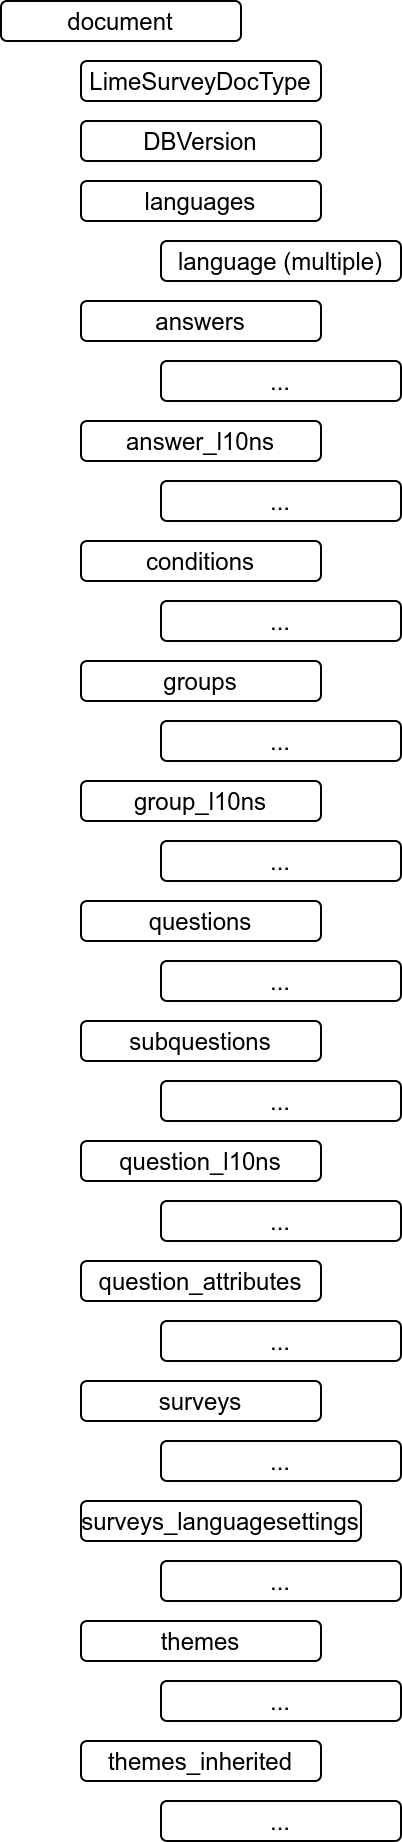
\includegraphics[width=.25\textwidth]{./img/append_lss.png}
			\caption{Aufbau des Wurzel-Elements \el{document}}
			\label{app:lss_struct}
\end{figure}

\begin{figure}[h]
	\centering
	\begin{subfigure}[b]{.45\textwidth}
		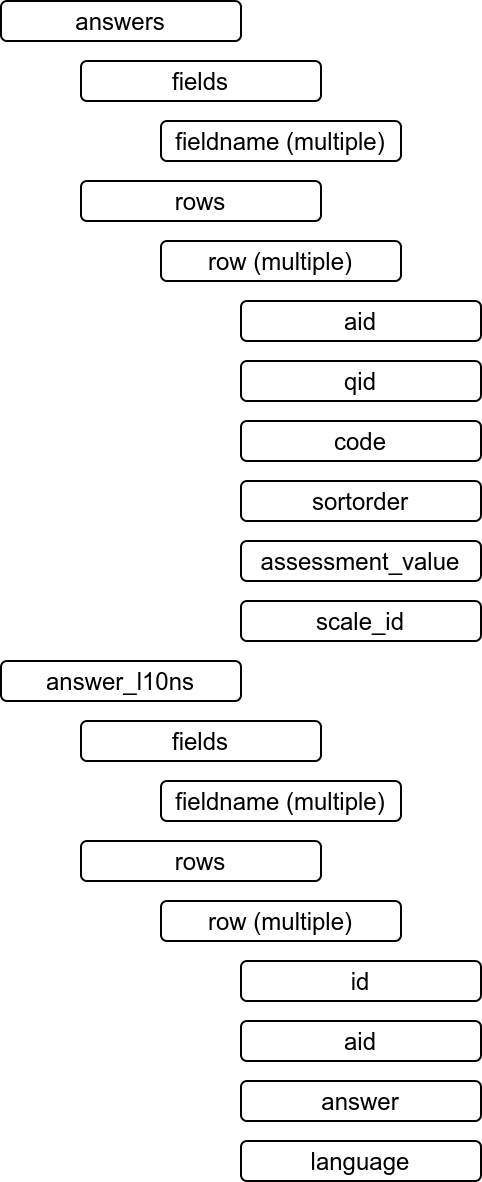
\includegraphics[width=.95\textwidth]{./img/append_lss_ans.png}
		\caption{Aufbau der Elemente für die Antworten}
	\end{subfigure}%
	\begin{minipage}[b]{.45\textwidth}
		\begin{subfigure}[b]{\linewidth}
			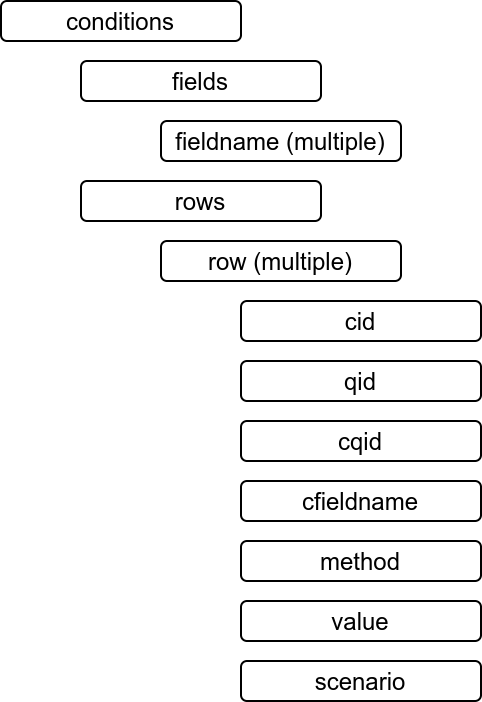
\includegraphics[width=.95\textwidth]{./img/append_lss_cond.png}
			\caption{Das Element für die Bedingungen}
		\end{subfigure}\\
		\begin{subfigure}[b]{\linewidth}
			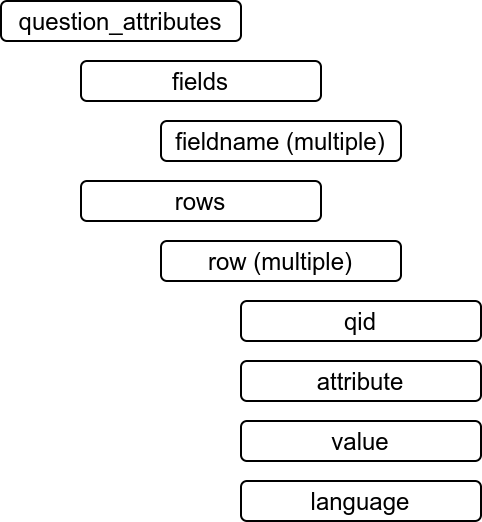
\includegraphics[width=.95\textwidth]{./img/append_lss_q_attr.png}
			\caption{Die Frageattribute im LSS-Format}
		\end{subfigure}%
	\end{minipage}
\end{figure}

\begin{figure}[h]
	\makebox[\linewidth][c]{%
		\begin{subfigure}[b]{.45\textwidth}
			\centering
			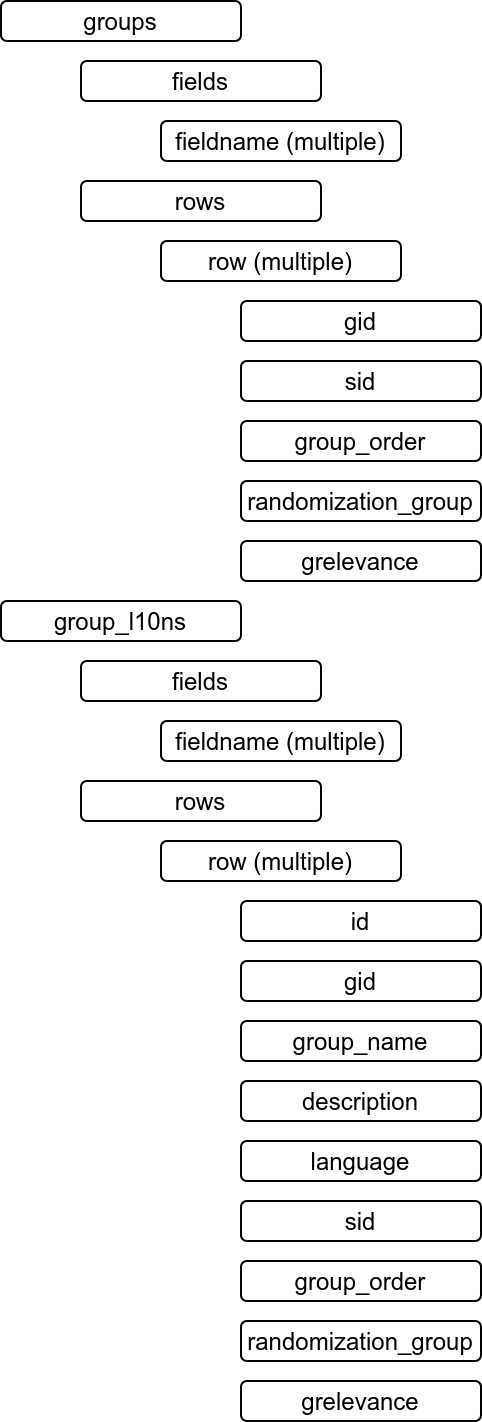
\includegraphics[width=.95\textwidth]{./img/append_lss_group.png}
			\caption{Aufbau von Fragegruppen}
		\end{subfigure}%
		\begin{subfigure}[b]{.45\textwidth}
			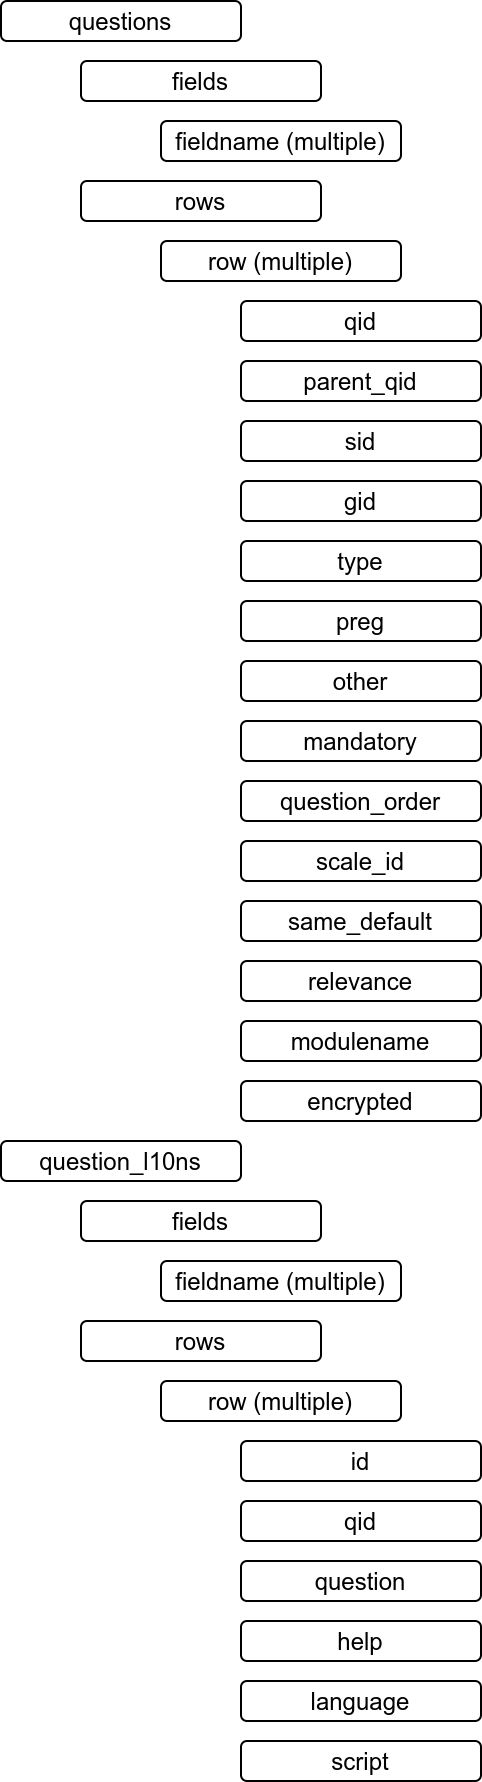
\includegraphics[width=.95\textwidth]{./img/append_lss_q.png}
			\caption{Aufbau der Frageelemente}
		\end{subfigure}%
		}
		\caption{Diagramme für Fragegruppen und Fragen}
\end{figure}

\begin{figure}[h]
	\centering
	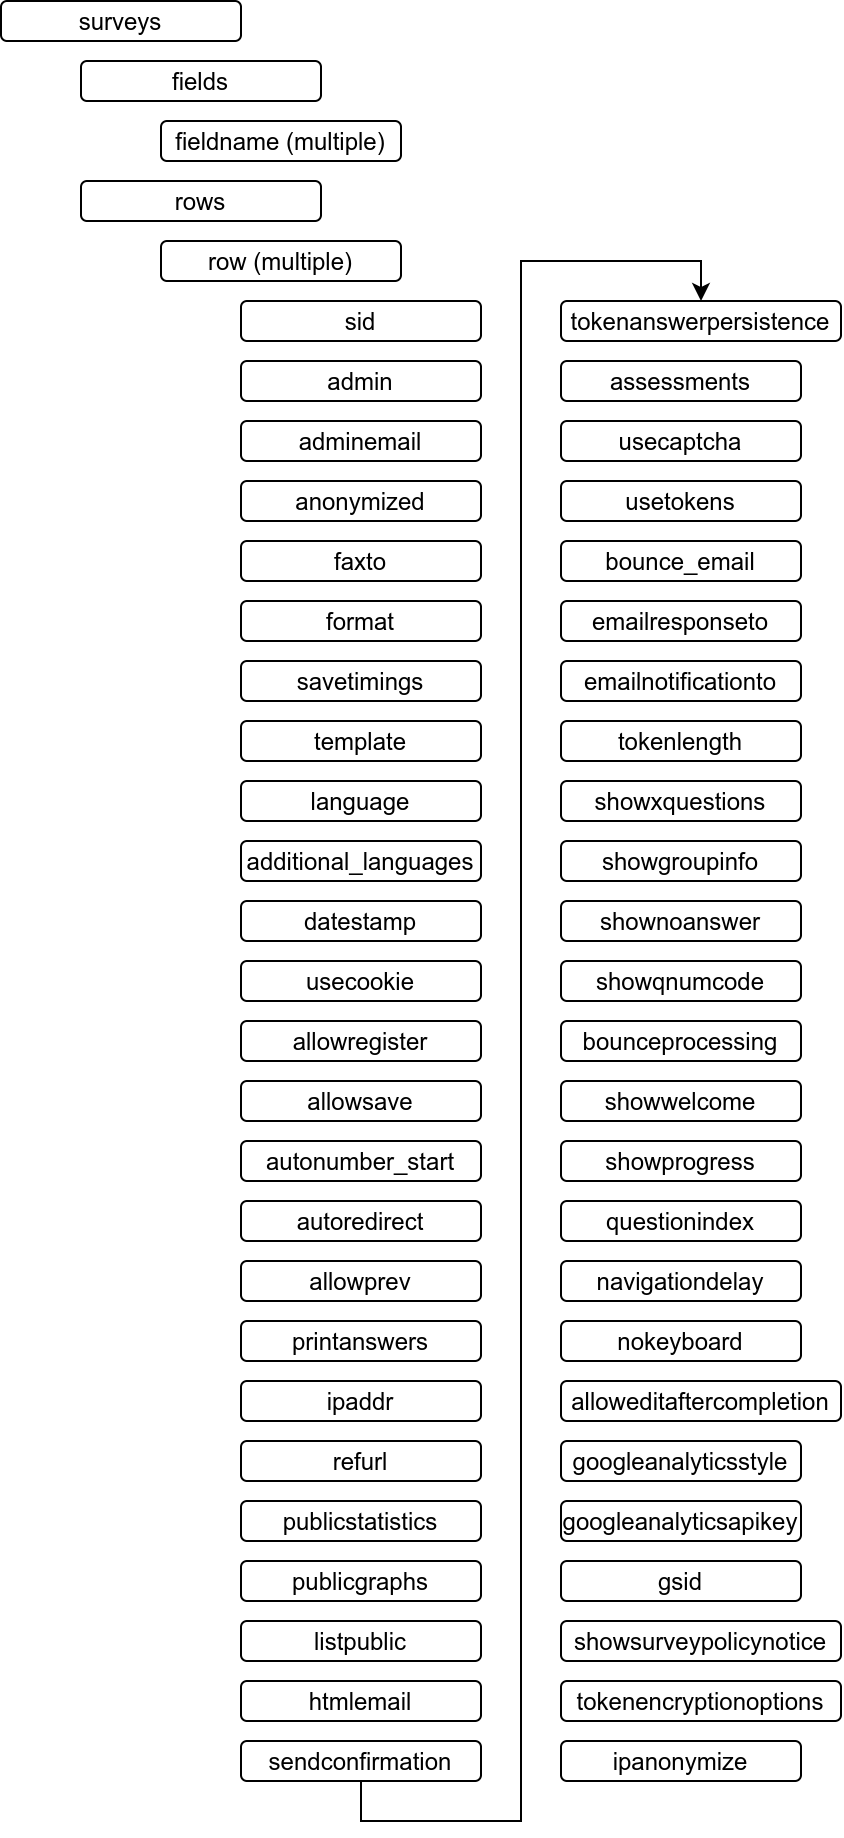
\includegraphics[width=.7\textwidth]{./img/append_lss_sur.png}
	\caption{Aufbau der Metadaten einer Umfrage}
\end{figure}

\begin{figure}[h]
	\makebox[\linewidth][c]{%
		\begin{subfigure}[b]{.45\textwidth}
			\centering
			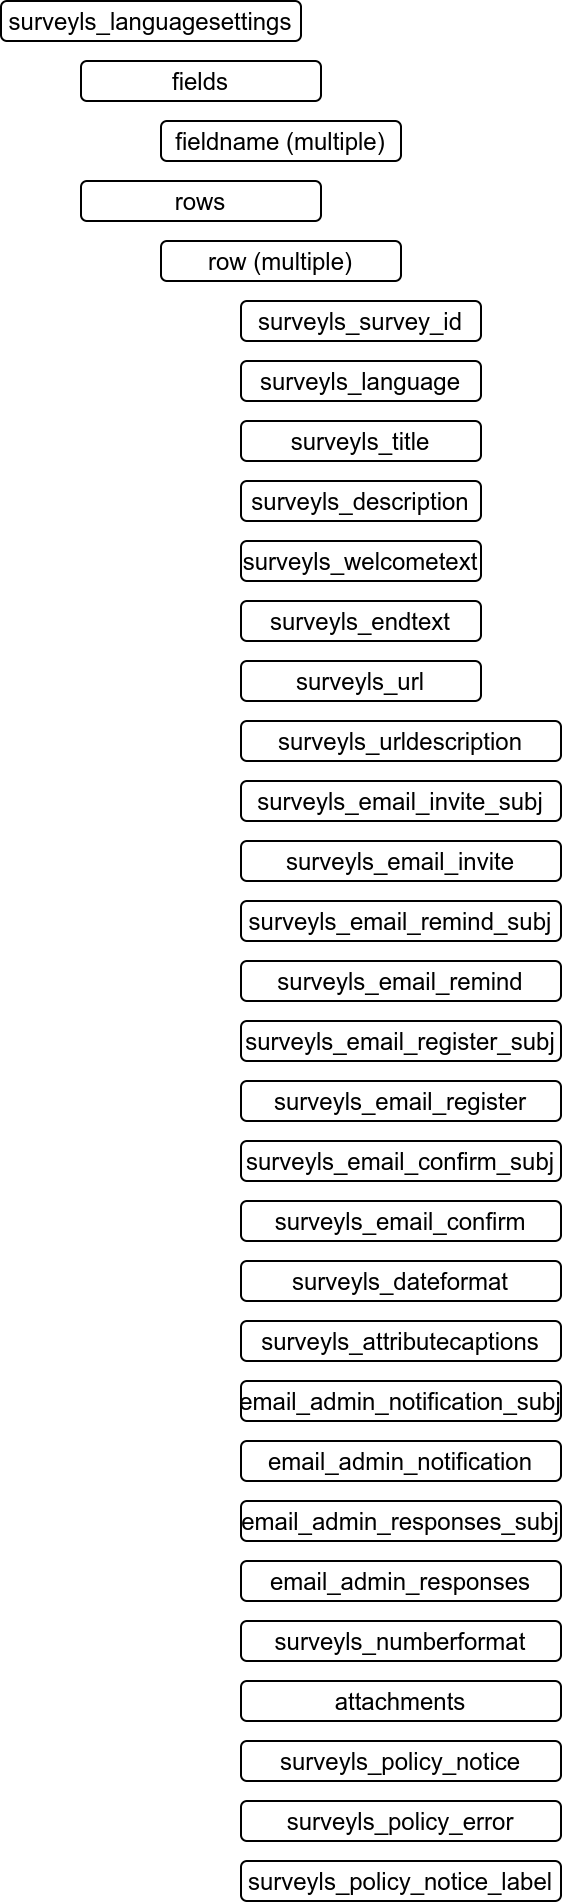
\includegraphics[width=.95\textwidth]{./img/append_lss_surls.png}
			\caption{Aufbau von weiteren Metadaten der Umfrage}
		\end{subfigure}%
		\begin{subfigure}[b]{.45\textwidth}
			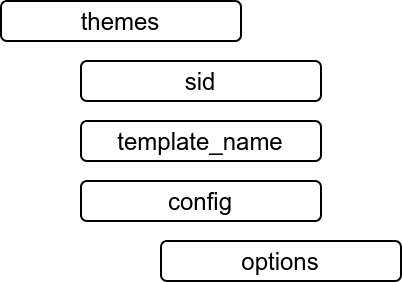
\includegraphics[width=.8\textwidth]{./img/append_lss_theme.png}
			\caption{Aufbau eines Themes}
		\end{subfigure}%
		}
		\caption{Diagramme für Metadaten der Umfrage und des Designs}
\end{figure}

\begin{figure}[h]
	\centering
	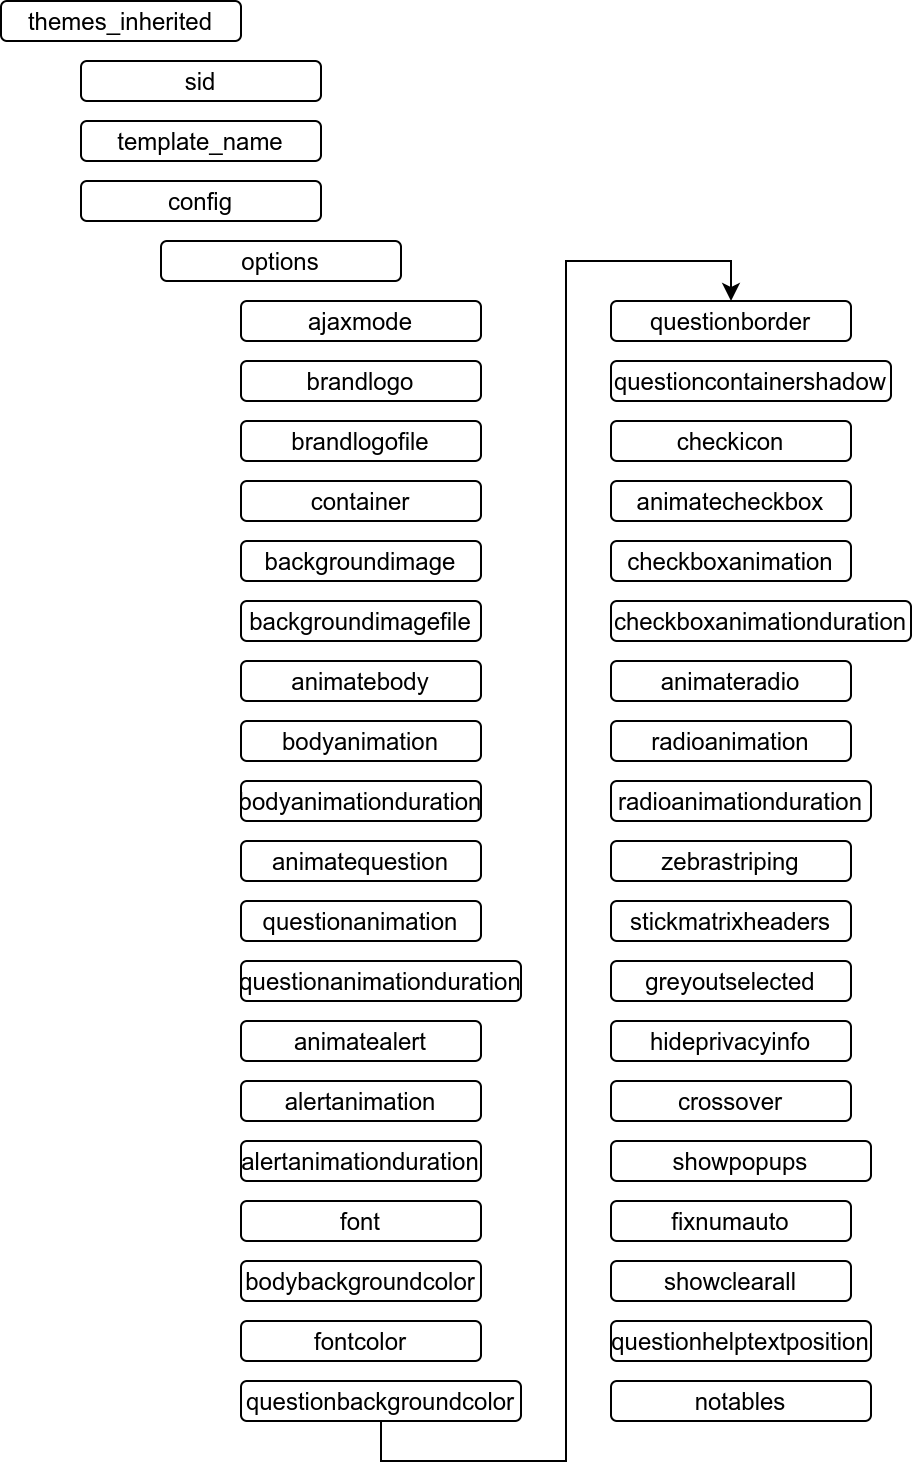
\includegraphics[width=.95\textwidth]{./img/append_lss_theme_inh.png}
	\caption{Aufbau der geerbten Designs}
\end{figure}

\chapter{Klassendiagramme des Programms lsa2odm}

\begin{figure}[h]
	\makebox[\linewidth][c]{%
		\begin{subfigure}[b]{.6\textwidth}
			\label{fig:app}
			\centering
			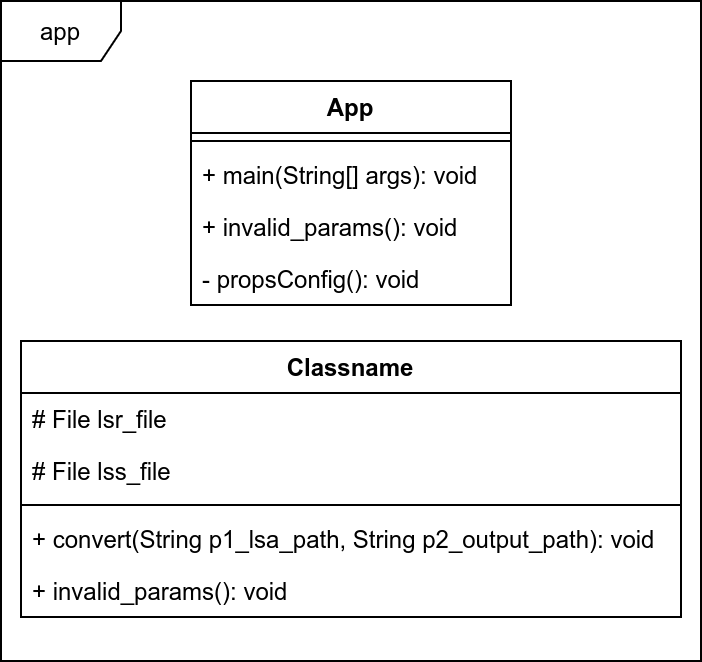
\includegraphics[width=.95\textwidth]{./img/cls_app.png}
			\caption{Klassendiagramm für das Paket \jv{app}}
		\end{subfigure}%
		\begin{subfigure}[b]{.6\textwidth}
			\label{fig:utils}
			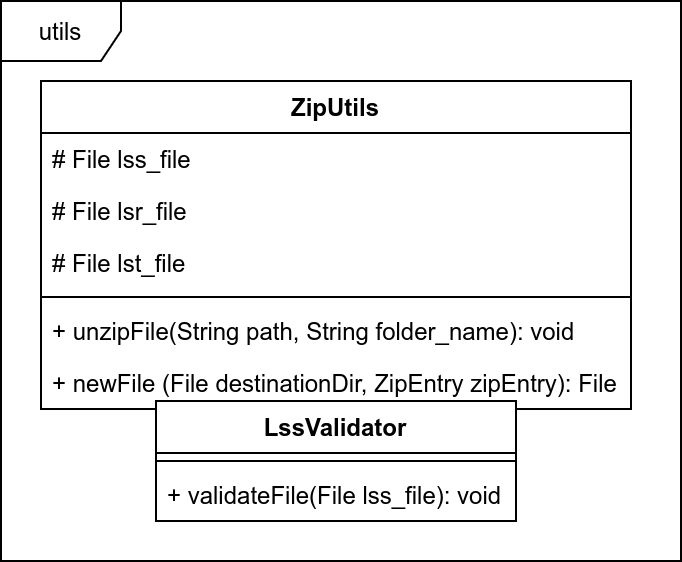
\includegraphics[width=.95\textwidth]{./img/cls_utils.png}
			\caption{Klassendiagramm für das Paket \jv{utils}}
		\end{subfigure}%
		}
		\caption{Klassendiagramme für mehrere Pakete, welche am Anfang der Ausführung gebraucht werden}
\end{figure}

\begin{figure}[h]
	\label{im:fig:lss}
	\centering
	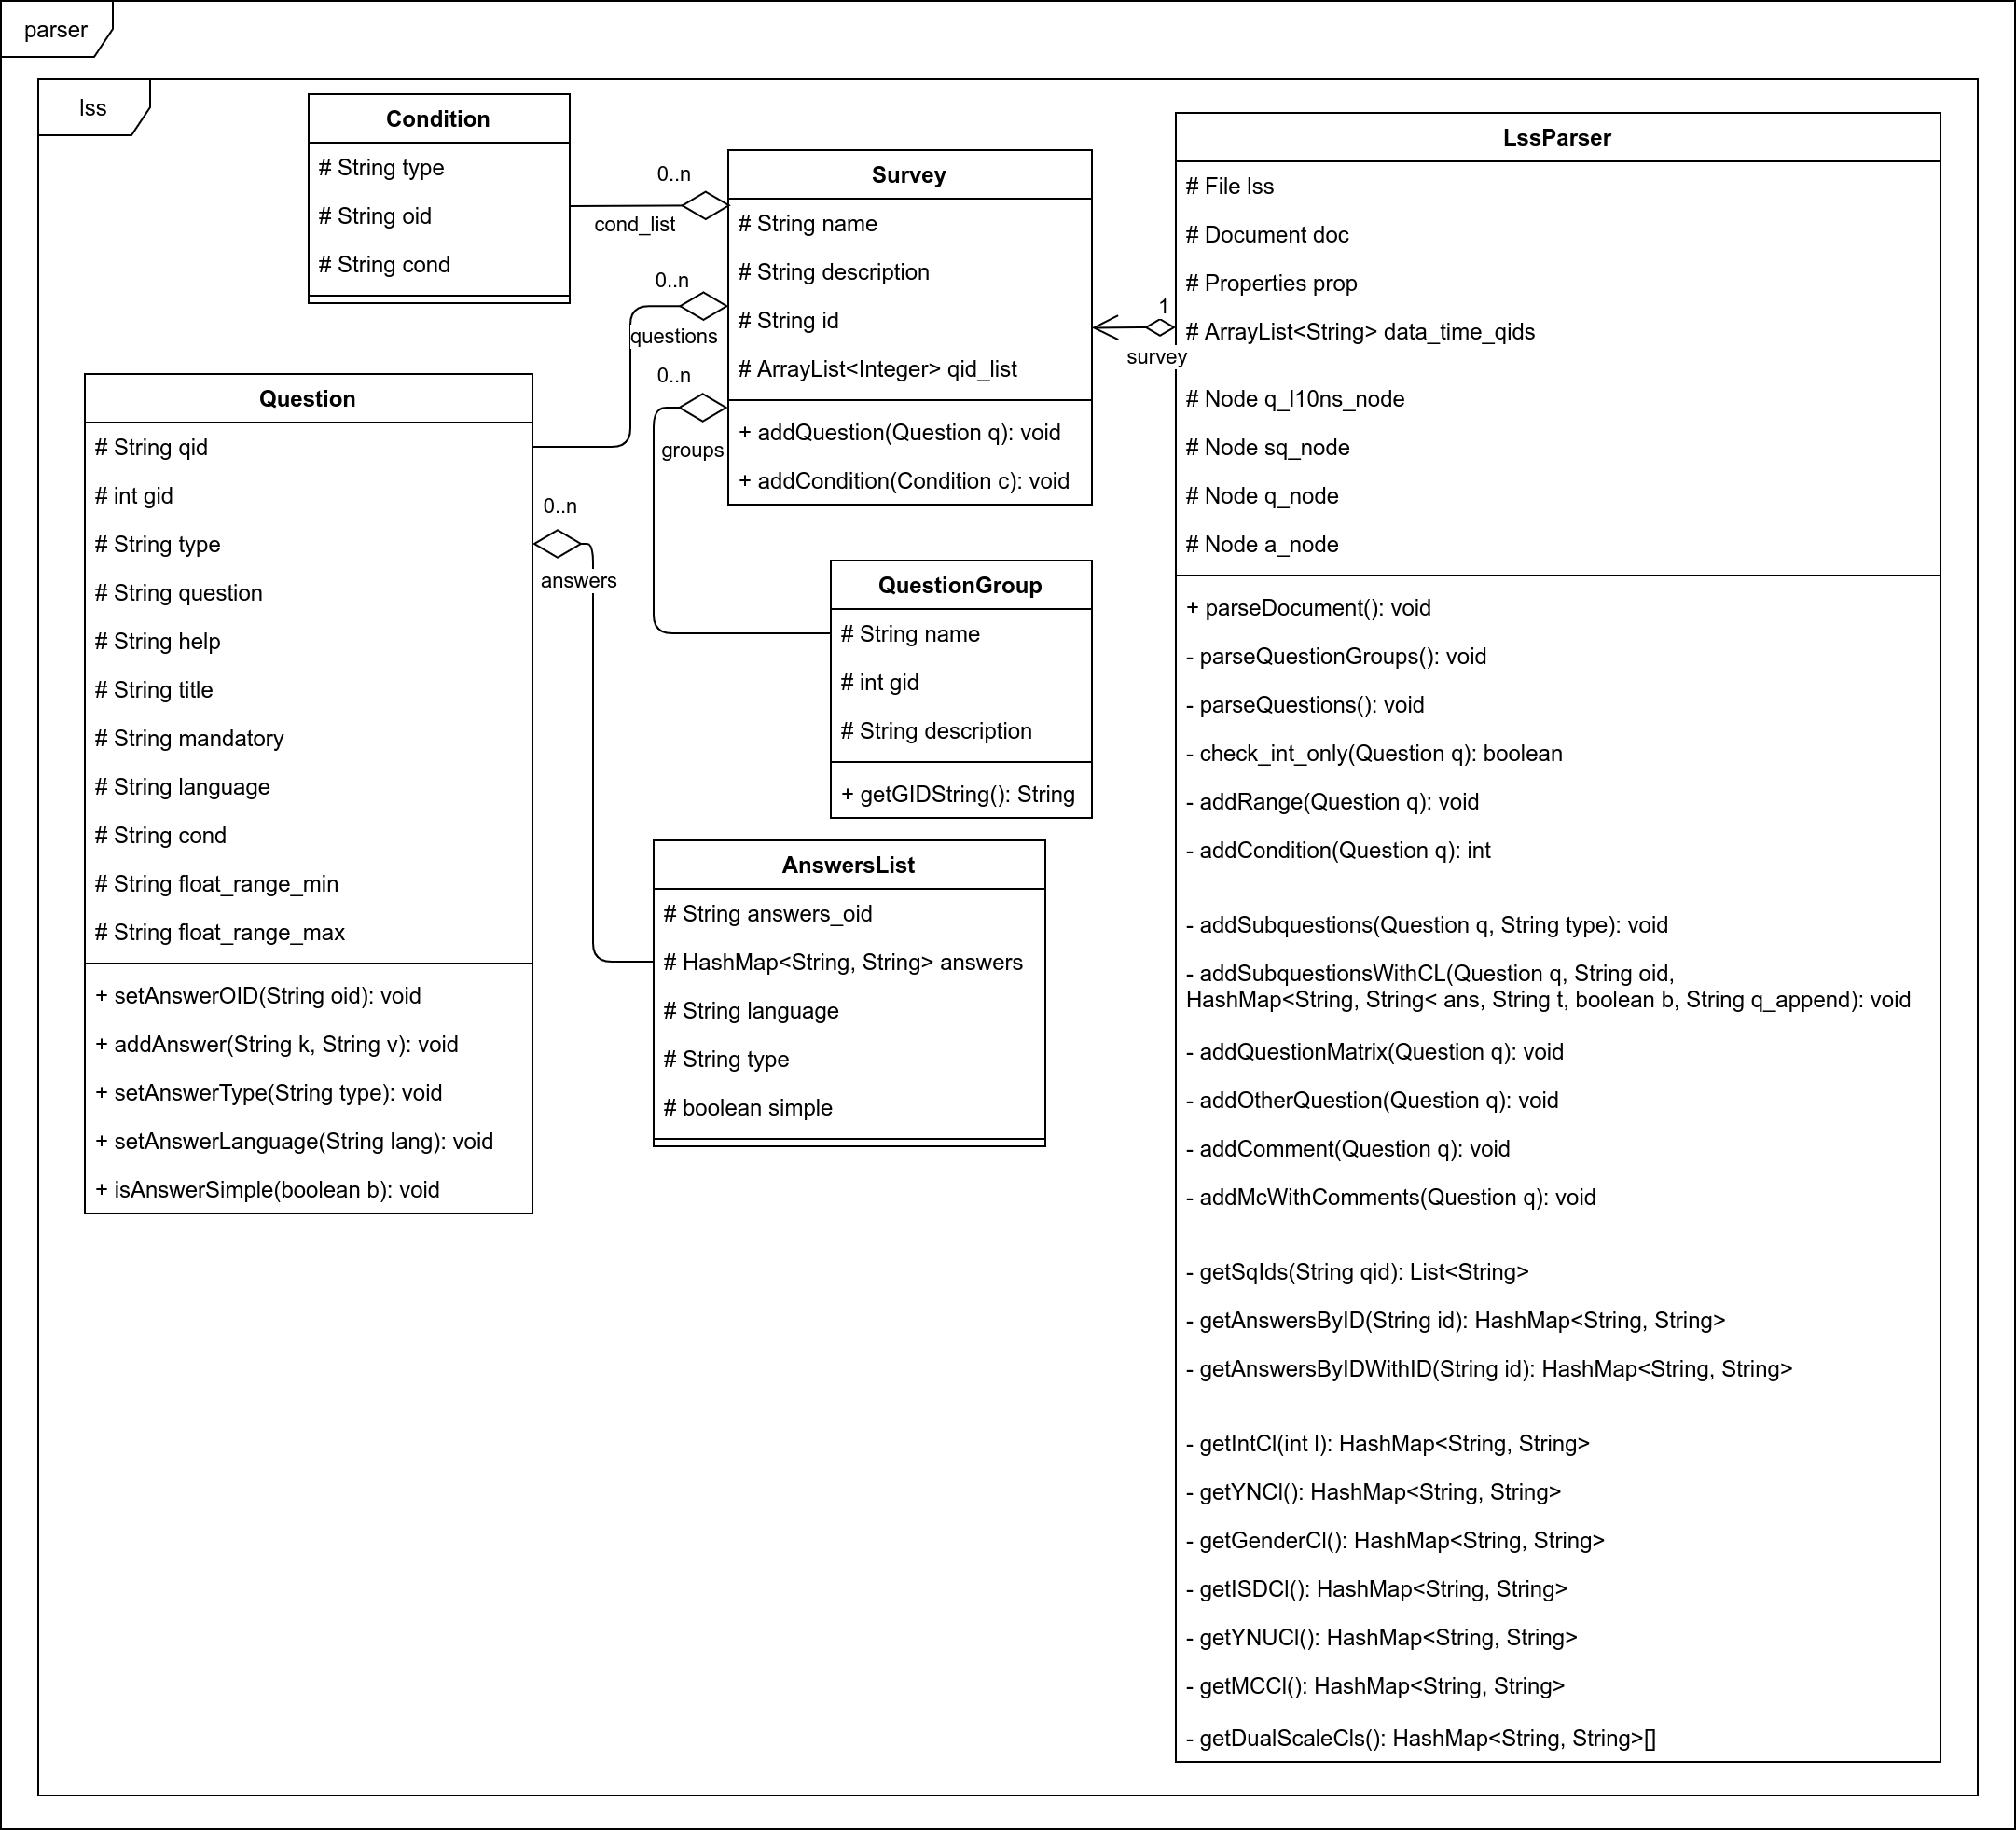
\includegraphics[width=0.90\textwidth]{./img/cls_lss.png}
	\caption{Klassendiagramm für das Paket \textit{lss}}
\end{figure}

\begin{figure}[t]
	\centering
	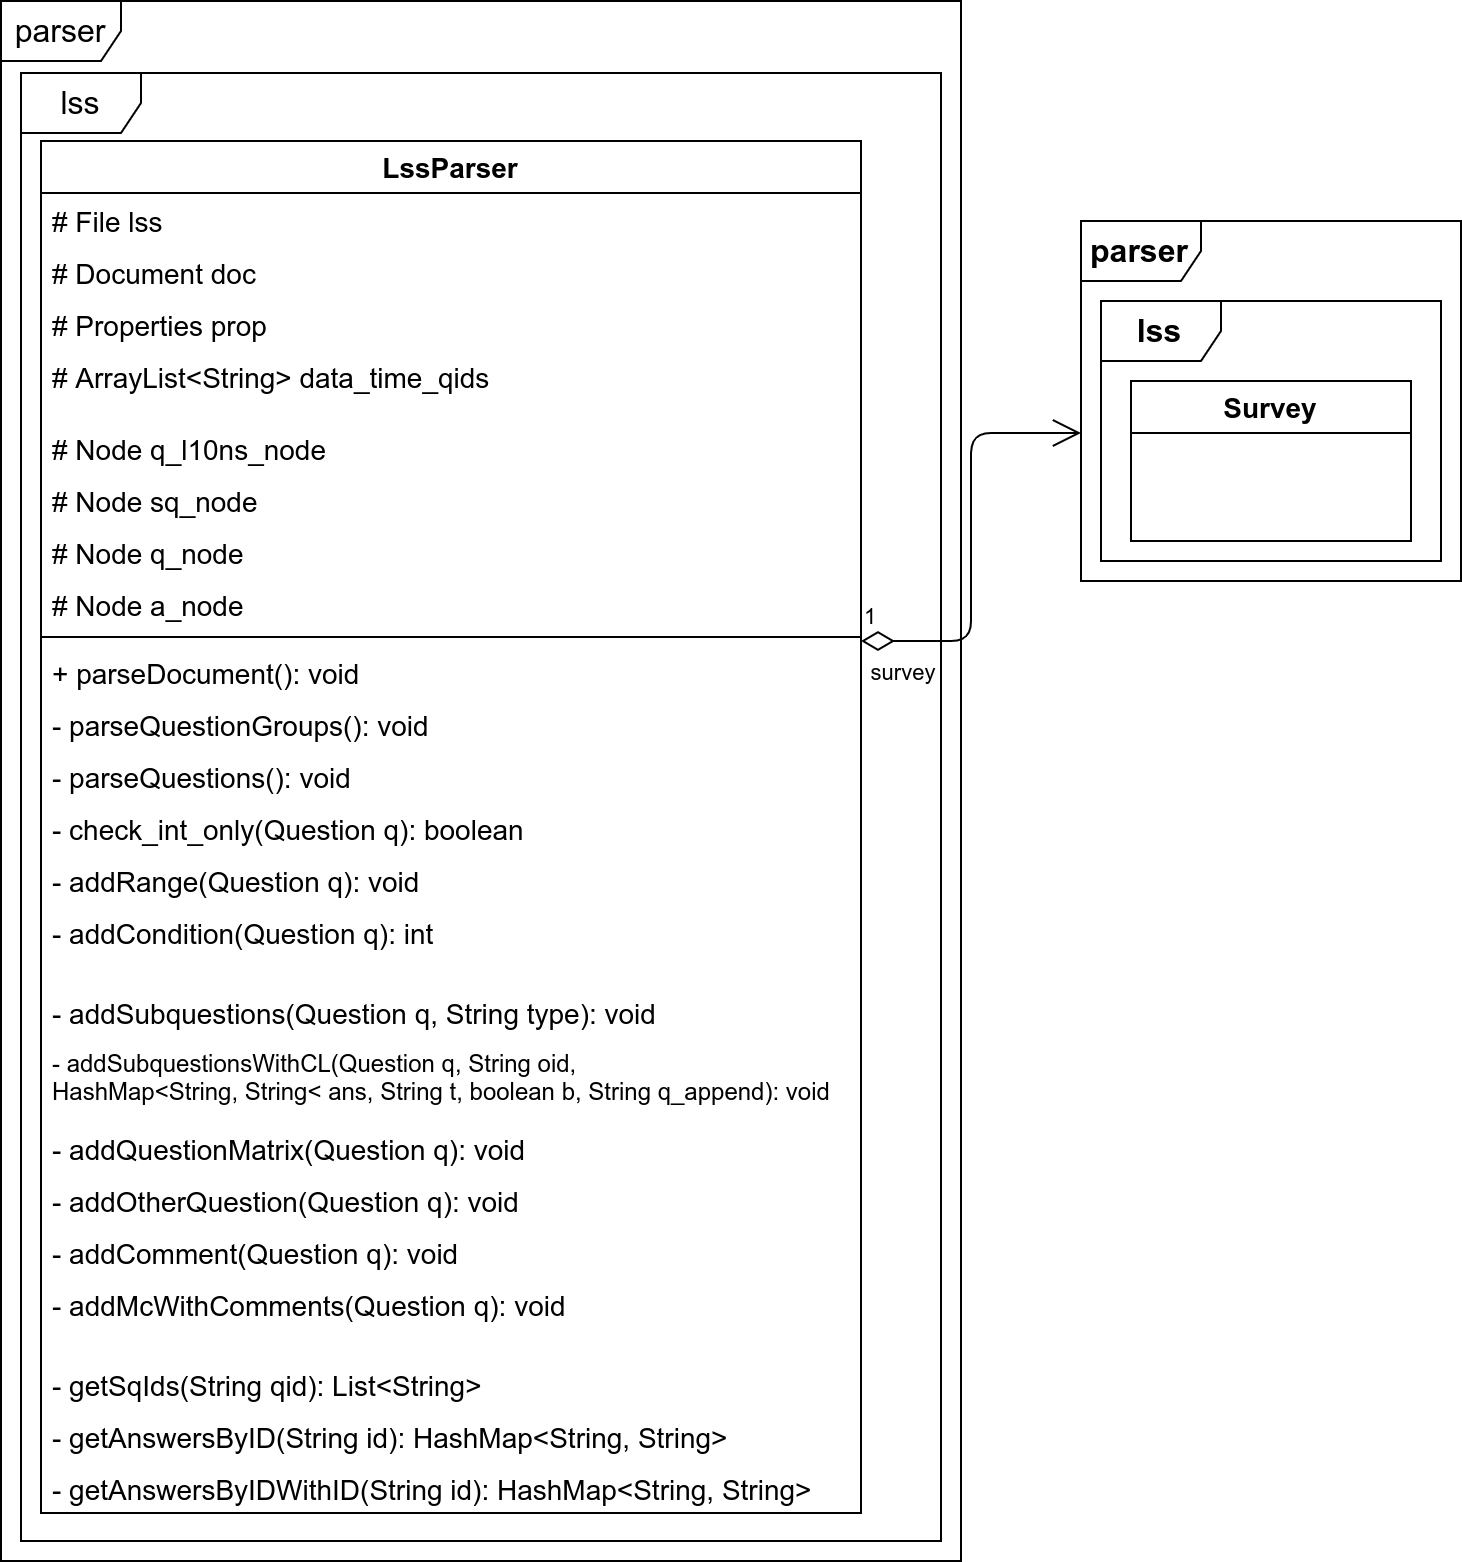
\includegraphics[width=0.99\textwidth]{./img/cls_lss_2.png}
	\caption{Klassendiagramm für \textit{LssParser}}
	\label{fig:lss2}
\end{figure}

\begin{figure}[h]
			\centering
			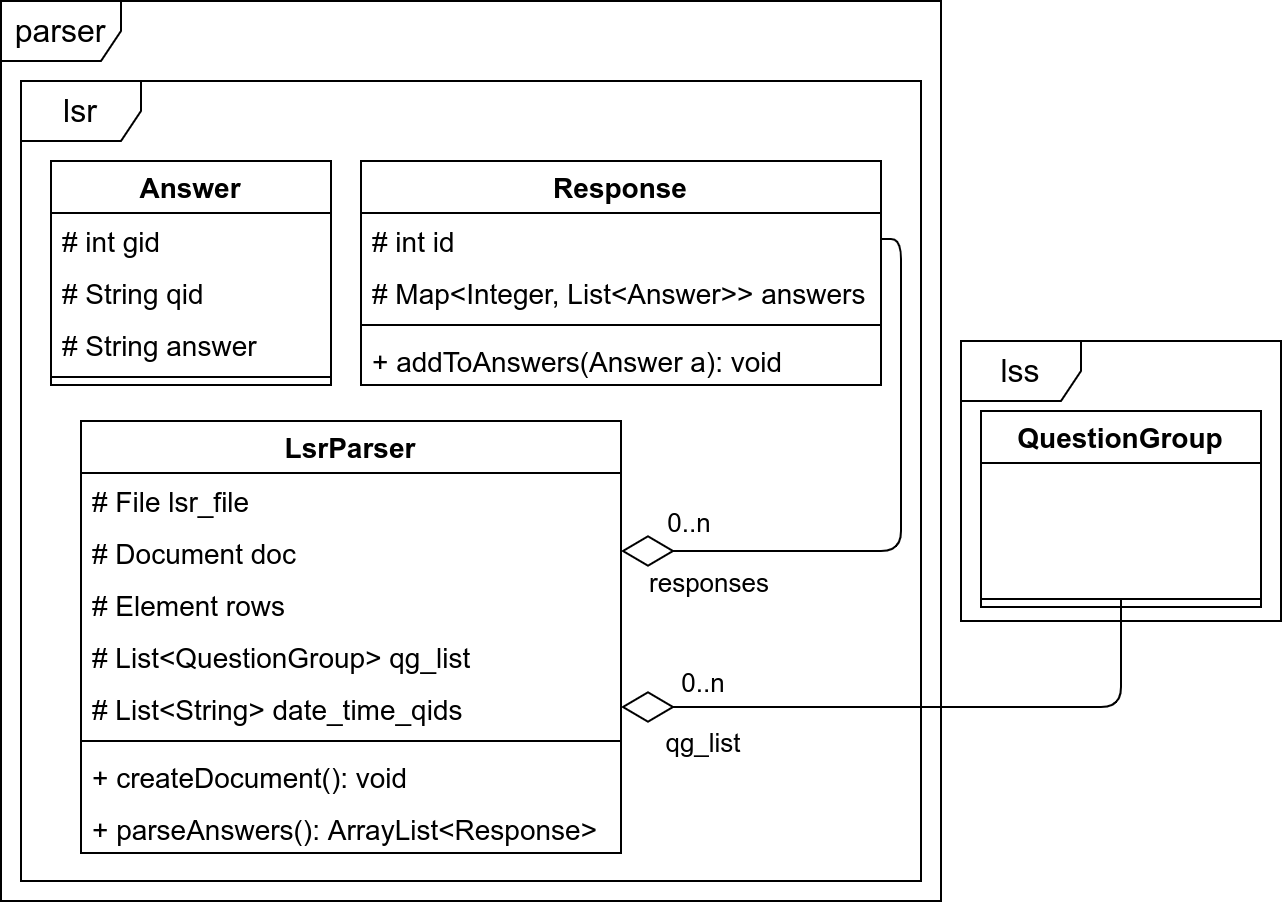
\includegraphics[width=.98\textwidth]{./img/cls_lsr.png}
			\caption{Klassendiagramm des Paketes \textit{lsr}}
\end{figure}

\begin{figure}[h]
	\centering
	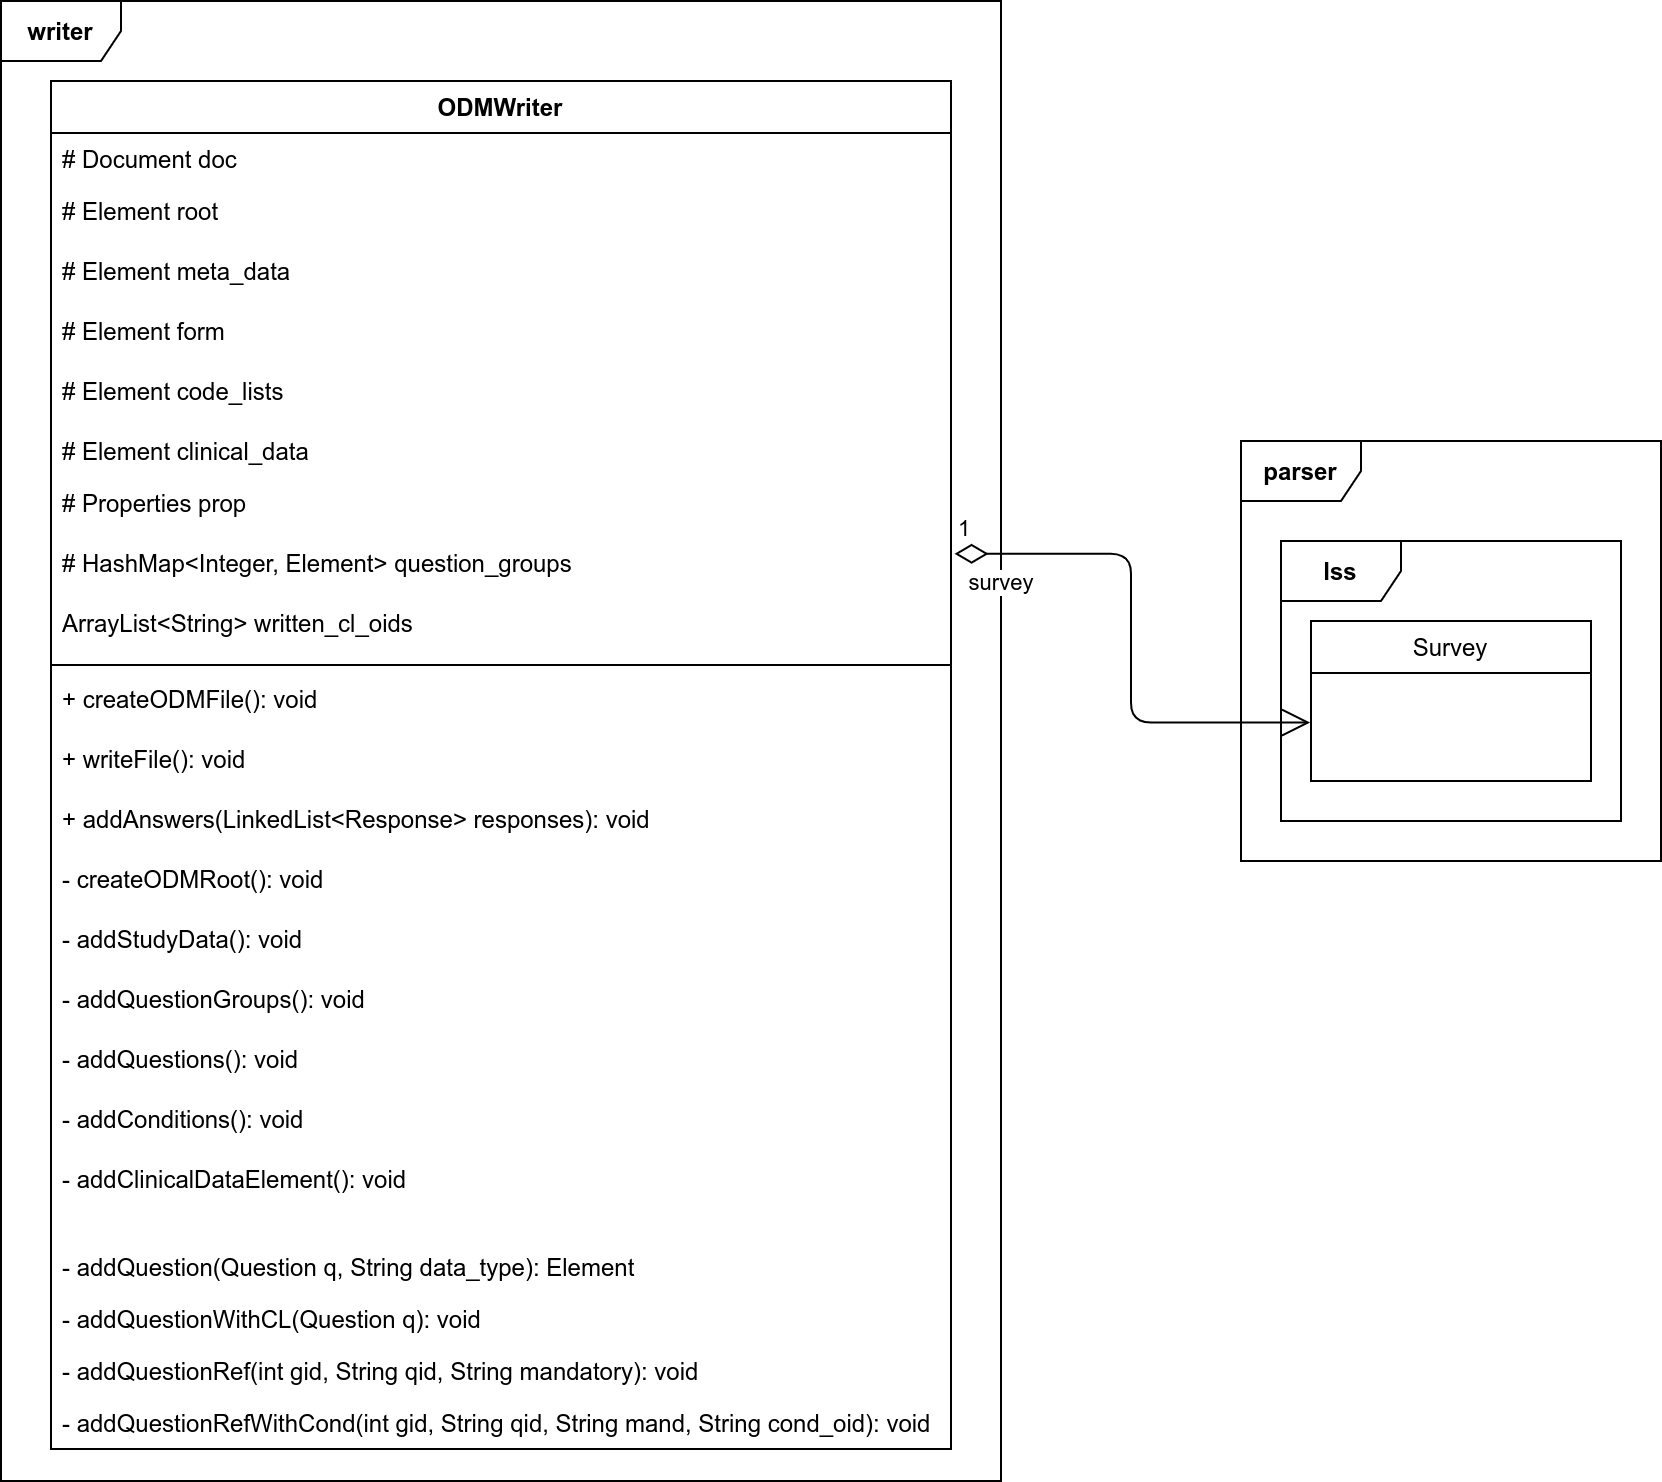
\includegraphics[width=.98\textwidth]{./img/cls_writer.png}
	\caption{Klassendiagramm des Pakets writer}
\end{figure}


% Literaturverzeichnis
% \bibliographystyle{unsrtdin}
% \bibliography{Quellen}
\printbibliography

\section{Akronyme}

\begin{description}[font=\sffamily\bfseries, leftmargin=0cm, itemsep=-0.15cm, style=nextline]
	\item \textbf{EDC} \el{Electronic Data Capture} Das Sammeln und Verarbeiten von Daten
	\item \textbf{RegEx} \el{Regular Expression} Ein Ausdruck, der genutzt werden kann, um Zeichenketten auf eine bestimmte Struktur zu überprüfen
	\item \textbf{IMI} \el{Institut für Medizinische Informatik} Eines der Institute der WWU. Diese Arbeit ist in Kooperation mit ihnen entstanden
	\item \textbf{XML} \el{eXtensible Markup Language} Eine Auszeichnungssprache zum Speichern hierarchisch strukturierter Daten 
	\item \textbf{XSD} \el{XML Schema Definition} Eine Datei, welche beschreibt, wie ein XML-Dokument aufgebaut sein sollte, um einer bestimmten Definition zu entsprechen.
	\item \textbf{SAX} \el{Simple API for XML} Ein Standard, welcher beschreibt, wie man ein XML-Dokument parsen kann. Dieses wird sequentiell eingelesen und für definierte Ereignisse wird eine vorgegebene Rückruf-Funktion aufgerufen. Ein Programm kann eigene Funktionen registrieren und so das Dokument verarbeiten.
	\item \textbf{DOM} \el{Document Object Model} Bietet die Möglichkeit, die Hierarchie der XML-Knoten in Baumform darzustellen und so zu navigieren/ den Baum zu bearbeiten
	\item \textbf{CDISC} \el{Clinical Data Interchange Standards Consortium} Eine Non-Profit-Organisation, welche Standards zum Austausch von Daten aus klinischen Studien entwickelt
	\item \textbf{CDISC ODM} \el{Operational Data Model} von CDISC entwickeltes XML-Format (siehe \cref{m:odm})
	\item \textbf{lsa} Abkürzung für und Dateiendung des LimeSurvey Archives (siehe \cref{m:lsa})
	\item \textbf{lsr} Abkürzung für und Dateiendung der LimeSurvey Response Datei (siehe \cref{m:lsa})
	\item \textbf{lss} Abkürzung für und Dateiendung der LimeSurvey Struktur Datei (siehe \cref{m:lsa})
\end{description}


% Eidesstattliche Erklärung
\chapter*{Eidesstattliche Erklärung}

% Die Aktuelle Version der Eidesstättlichen Erklärung kann beim zuständigen Prüfungsamts gefunden werden.
% Nachfolgend ist die Version für Bachelor und Master des Prüfungsamts Mathe/Informatik vom 05.10.2016

Hiermit versichere ich, dass die vorliegende Arbeit über \textit{\glqq Titel\grqq} selbstständig verfasst worden ist, dass keine anderen Quellen und Hilfsmittel als die angegebenen benutzt worden sind und dass die Stellen der Arbeit, die anderen Werken – auch elektronischen Medien – dem Wortlaut oder Sinn nach entnommen wurden, auf jeden Fall unter Angabe der Quelle als Entlehnung kenntlich gemacht worden sind.

\vspace{1cm}

\parbox{20em}{\hrulefill}

Vorname Nachname, Münster, \today

\vspace{1cm}

Ich erkläre mich mit einem Abgleich der Arbeit mit anderen Texten zwecks Auffindung von Übereinstimmungen sowie mit einer zu diesem Zweck vorzunehmenden Speicherung der Arbeit in eine Datenbank einverstanden.

\vspace{1cm}

\parbox{20em}{\hrulefill}

Vorname Nachname, Münster, \today

\end{document}
